%
%--- Este documento estrutura o projeto do ALUNO-1
%

%\input{/home/elias/work/defs/defs}
\documentclass[12pt,brazil,english]{abnt}
%\documentclass[12pt,brazil]{abnt}
\usepackage{babel,graphicx,verbatim,abnt-alf,enumerate,lineno}
\usepackage{pstricks,pst-node}
%\usepackage[latin1]{inputenc}
%\usepackage{apalike}
\usepackage{setspace}
\usepackage{float}
%\usepackage{subfig}
\usepackage{algorithmic}
\usepackage{algorithm}
\usepackage{multirow}
\usepackage{color}

\usepackage[brazil]{varioref}

%\usepackage{pdflatex}
%\usepackage[pdftex]{graphicx}

\usepackage[T1]{fontenc}
\usepackage{psfrag}
\usepackage{graphicx}

%\usepackage[a4paper,top=30mm,bottom=30mm,left=30mm,right=25mm]{geometry}
%\geometry{headheight=7mm,headsep=3mm,footskip=7mm}
%\setlength{\parskip}{2ex plus0.5ex minus0.5ex}
% Espa�amento 1.5, requerido pelo PPGEE. O valor de \baselinestretch
% foi extraido do ``LaTeX Companion'', pp. 52-53.
%\renewcommand{\baselinestretch}{1.21}

\usepackage{epic,eepic}
\usepackage{amssymb,calc,url,indentfirst,enumerate,theorem,moreverb}
\usepackage{alltt,fancyhdr,subfig,tabularx}

\begin{document}
%\pagewiselinenumbers %--- Set line numbering 

\pagestyle{empty}

%\begin{abstract}
%
% O resumo deve conceituar o projeto com seus objetivos e justificativas
% ou evid�ncias de interesse.
%
%\input{abstract-pt}
%\end{abstract}

\DeclareGraphicsRule{.eps.gz}{eps}{.eps.bb}{`gunzip -c #1}
\graphicspath{{figuras/}}

\autor{Lucas de Paula Veronese}


\titulo{Autonomous Cars Localization in GPS-Denied Urban Environments using Road and Satellite Maps}


\orientador{Prof. Dr. Alberto Ferreira De Souza}


%\coorientador{<Nome do Co-orientador (caso exista)>}


\comentario{Tese apresentada ao Programa de P�s-Gradua��o em Inform�tica do Centro Tecnol�gico da Universidade Federal do Esp�rito Santo, como requisito parcial para obten��o do Grau de Doutor em Ci�ncia da Computa��o.}


\instituicao{Departamento de Inform�tica \par Centro Tecnol�gico\par Universidade
Federal do Esp�rito Santo}


\local{Vit�ria - ES, Brasil}


\data{}

\capa

\folhaderosto

\begin{folhadeaprovacao}
%Tese apresentada ao Programa de P�s-Gradua��o sob o t�tulo \textit{``\ABNTtitulodata''},
%defendida por \ABNTautordata~e aprovada em \ABNTdatadata, em Vit�ria,
%Estado do Esp�rito Santo, pela banca examinadora constitu�da pelos
%professores: 
\setlength{\ABNTsignthickness}{0.4pt}

\assinatura{Prof. Dr. Alberto Ferreira De Souza\\ Orientador} \assinatura{Prof. Dr. Edilson de Aguiar \\ Co-orientador} \assinatura{Prof. Dr. Thiago Oliveira dos Santos\\ Universidade Federal do Esp�rito Santo} \assinatura{Prof. Dr. Claudine Badue\\ Universidade Federal do Esp�rito Santo} \assinatura{Prof. Dr. Fernando A. Auat Cheein\\ Universidad T�cnica Federico Santa Mar�a}  \assinatura{Prof. Dr. Jos� Guivant\\ University of New South Wales}
\end{folhadeaprovacao}
%\begin{resumo}
%Escreva aqui o texto do seu resumo.
%\end{resumo}

\chapter*{Resumo}

resumo

\begin{abstract}
Write here the English version of your {}``Resumo''.
\end{abstract}


\chapter*{Dedicatory}

Dedico este trabalho a ...


\chapter*{Acknowledgment}

Agrade�o a ...



\tableofcontents{}\listoffigures

\listoftables


\chapter{Introduction}
\label{cap:Introductions}

Accurate global localization is a necessary capability of autonomous vehicles intended to operate in large areas. In many cases, the context of operation does not allow the use of GPS, or degraded GPS estimates makes its direct use inappropriate (e.g. urban canyons, hostile territories in war scenarios, underground mines, etc.). Alternative localization mechanisms, such as those based on SLAM \cite{42montemerlo2007fastslam, 08weingarten2005ekf, 37auat2011optimized, 10thrun2006graph}, require the vehicle to “close the loop” (revisit places) for maintaining the required accuracy, what, in certain cases, is not possible because the vehicle’s plans do not actually involve revisiting places. Approaches based on detailed a priori maps (\cite{Thrun00j, Levinson-RSS-07, LevinsonT10, ranganathan2013light}) are also possible, but require building its map in advance (usually by visiting and learning the context of operation).

One viable alternative can be implemented using information publically available in the form of road maps and on-board sensing capabilities that comes today as standard in most cars. These sensing capabilities allow easy implementation of dead-reckoning (at least low quality dead-reckoning) and of some level of environment modelling.

Based on those resources, a Bayesian estimation process can be performed in order to estimate the global pose (position and heading) of the platform. In the estimation process, the kinematic model of the vehicle can be used as a Process Model. The road map is used to define the main observation model (i.e. a likelihood function), based on the assumption that the vehicle is usually located on a known road. The additional sensing capabilities can offer extra observations for improving the convergence of the estimation process (what is the case presented in this work).

As the generated Probability Density Function (PDF) for describing the estimates (2D position or 3DoF Pose) is usually non Gaussian, the Bayesian estimation process is usually implemented through approaches such as Particle Filter (PF) or Sum of Gaussians (SoG). An approach for implementing such an estimation process was introduced  in \cite{guivant2007global} and \cite{guivant2010robust}. In that approach, an extended likelihood function was defined to improve the performance of the PF estimation process. The approach was adequate for treating cases where the road map was only partially known (e.g. incomplete). However, it was noted that the quality of the estimates could be degraded in certain operation conditions. Those conditions occur when the vehicle travels for large distances throughout almost rectilinear roads, i.e. when it does not turn at any intersection for long distances. That behavior could affect the observability of the estimation process, increasing the uncertainty on the longitudinal component of the position estimates. 

Those situations suggest the need of using additional observations that could provide information related to the longitudinal component of the vehicle position. Particular cases where such observations are possible occur in the vicinity of known road intersections, even when the vehicle does not turn and keep going straight. From the detection of such cases, an associated likelihood function could be generated and used for updating the estimation process. In this paper, a new class of observation based on the detection of intersections in road maps is defined, and the verified improvements in our previous algorithm \cite{guivant2007global} are shown via experiments with an autonomous car.
This work is organized as follows. After this introduction, in Section II, we briefly present the related work. In Section III, we describe our Localization System. Thereafter, in Section IV, we present our experimental setup and our experimental methodology. Section V presents the results, and our conclusions follow in Section VI.


Mapping large-scale environments is still a challenging problem (\cite{60kummerle2009autonomous,61sunderhauf2012switchable,68mcdonald2013real}), especially in environments with loop closures separated by long distances. It is to be noted that related works on the topic (as will be shown in the following Section) are typically only focused in one specific type of environment, meaning: outdoors, indoors, urban or agriculture. They do not face the problem of environment transitions (from indoors to outdoors, from urban to highly arborized, among other possible combinations). The latter is the main contribution of this article, since we implement and evaluate a GraphSLAM-based algorithm for mapping in the following complex field scenarios: downtown of an urban region, arborized university campus and their corresponding transitions, using an autonomous car. The map built by the system is used for localization and for autonomous navigation as the vehicle drives through the environments. A low level obstacle detection approach is also implemented in order to evaluate collision possibilities.

Additionally, in this work we also propose a new approach for estimation and integration of sensorial biases present in odometry data; the description of an end-to-end Large-Scale Mapping System based on GraphSLAM. This solution integrates data from odometry, IMU, GPS and Velodyne in a probabilistic path estimator; a new description of a Velodyne-based 2D grid-mapping algorithm, which was already presented by other authors \cite{22montemerlo2008junior} with a different description approach. In addition, we empirically show that the mapping system is able to build high quality maps of large-scale environments, including in presence of transitions between peripheral highly arborized areas and urban downtown areas.

The Large-scale Environment Mapping System (LEMS) was evaluated using the robotic vehicle (see Figure ~\ref{Fig::FIGURE01}) named IARA (acronym to Intelligent Autonomous Robotic Automobile), a robotized car from \emph{Universidade Federal do Esp\'irito Santo}, Brazil, in three environments with different scales and characteristics. The LEMS was successfully used to map all of them, with precise loop closures and without map drifts.

\begin{figure}[ht]
    \centering
    \includegraphics[scale = 0.1]{FIGURE01}
    \caption{Robotic platform named IARA (acronym to Intelligent Autonomous Robotic Automobile).}
    \label{Fig::FIGURE01}
\end{figure}

Localization and tracking of vehicles or robots in GPS-denied environments - both indoors and outdoors - is still challenging, specially when precise motion is required. A common solution is the use of Simultaneous Localization And Mapping (SLAM) algorithms.  However, such algorithms require the need of a robot initialization step. For instance, in an indoor environment, localizing a mobile robot using SLAM will depend on the place where it is initialized, i.e. where it wakes up.  This methodology is inefficient for some applications because the positions of the objects in the world will change depending on the initialization position.  A common solution to overcome this limitation is the construction of a map of the environment~\cite{Thrun00j,moreno2007evolutionary,bashiri2012hybrid}. For mapped environments, during the initialization step, the robot localizes itself according to the map, thus preserving the position of the objects in the world. Unfortunately, this additional step increases the 
computational cost when the map grows. Furthermore, if the map has some ambiguity, finding the robot pose may take a few minutes.



\section{Motivation}

\section{Contribution}

\section{Structure}


\chapter{Related Work}

Robot localization and mapping has been treated as fundamental problem in robotics filed. In general, they are addressed as Simultaneous Localization And Mapping (SLAM)  \cite{guivant2012internet, robledo2011outdoor, lohrsemantic, 58segal2009generalized,42montemerlo2007fastslam, 08weingarten2005ekf}. I.e., while the robot is navigating and planning its movements to avoid obstacles, it maps the environment and localizes itself using the map. The main disadvantage of online SLAM algorithms is the inability to revisit sensors data, in special to handle the loop closure problem \cite{10thrun2006graph}.

Therefore, a Graph-SLAM has been considering since it has a natural way to handle with loop closure problem \cite{10thrun2006graph, Levinson-RSS-07, LevinsonT10}, [15]. The Graph-SLAM algorithm proposed in \cite{10thrun2006graph} is a Full-SLAM algorithm that uses the whole sensor data to estimate the robot path and the map. In the Graph-SLAM, the nodes represent model variables (poses and map variables) and the edges represent sensors measurements and its respective covariance. However, the number of landmark in large outdoors areas tends to be huge being computationally unfeasible deal with this amount of data during the path optimization. Therefore, mapping large scale urban scenarios is addressed marginalizing the map variables to become restriction between poses \cite{Levinson-RSS-07, LevinsonT10}. 

Graph-SLAM algorithms are inherent offline, hence, to localize a robot during its navigation a Monte Carlo Localization or Kalman Filter based Localization must be considered \cite{Thrun00j}, [16]. Generally, to build the map in outdoor huge areas a GPS, IMU, robot odometry, and LiDAR are used. The main advantage of the use GPS is because it has limited error that never grows while the robot is moving. Nevertheless, the GPS signal suffers from outages or occlusions problems, which are intensified in places such as urban canyons, indoor places, underground mines, etc.

To overcome the issues in GPS denied places, in [15] they used available aerial photography as a map to localize the robot just once in the course, and generate the graph nodes by the localization returned poses. Thereafter, a Graph-SLAM is applied to produce the most likely path that will be used in the mapping. The alternative to perform the localization by using aerial map images is also used as the main localization of the robot in outdoor environment [17]–[20]. However, it fails when robotic vehicles are crossing tunnel or in a place with roof of trees. Moreover, in a featureless environment like mines, it would not work.

Alternatively, the road-map can be used to perform the robot localization in these GPS denied sites. Therefore, the road-map has been used to address the global localization problem \cite{guivant2007global,guivant2010robust}, [21]. In [21] they used the OpenStreetMap to globally localize a vehicle in unban roads. They do so, comparing the short historical of the visual odometry [22] against to the road-map using Monte Carlo Localization. In the proposals presented in \cite{guivant2007global, guivant2010robust}, rather than visual odometry, they use 200 meters of the vehicle dead-reckoning to perform the same pose correction. In those solutions, the robot position belief is high during the robot turn, but in a straight line the covariance can increase causing miss localization. 

One common feature in road-maps is the intersection between roads. Thereby, in this work, we are exploring this characteristic to reduce the position uncertainty in the car position. To perform the intersection detection a 3D LiDAR has been used to create a local map of environment. The local map is used to measure the road width. If the width is bigger than a threshold the car is on a road intersection.

Since the dead-reckoning is used to compare against the road-map to perform the particle correction in Monte Carlo localization, as well as to build the local map. Wheel slips 
during the car acceleration, turn and breaking may affect negatively the pose correction and also the local map construction. Thus, in this work, it has been corrected by scan-matching algorithm like Generalized Iterative Closest Point (well known as Generalized-ICP) in the case of this work [23].


After the Darpa Urban Challenge \cite{DBLP:conf/darpa/2009},  the automotive industry has increased the efforts to develop an autonomous vehicle. Most of the solutions depend on a good GPS receiver to localize the vehicles globally and absolutely, mainly for outdoor environments~\cite{bacha2008odin,leonard2008perception,Montemerlo:2008:JSE:1405647.1405651,Urmson:2008:ADU:1395073.1395077,Auat2013}. However, standard GPS signal is not always reliable when navigating on the roads or for indoor environments. To solve this problem, the approach proposed by the \emph{Stanford autonomous vehicle} used a map, built beforehand, to localize the car in the environment~\cite{Levinson-RSS-07,LevinsonT10}. The map is constructed using a Graph-SLAM algorithm fusing the data from the GPS, the IMU, the wheels odometry and the LiDAR. This way, when the GPS signal failed, a continuous localization could still be done using the other sensors.  However, it is not clear if the Graph-SLAM algorithm could be applied to GPS-denied 
environments, like a stockyard, a parking lot, and industrial plants. Other issue is how to perform the initial localization, i.e. the vehicle initialization, without a GPS signal. In addition, agricultural processes and the mining industry would also benefit from a GPS-independent but reliable localization system, as mentioned in~\cite{Auat2013}.
There is a high expectation that, in the future, autonomous vehicles will be used to provide accessibility to injured people, reduce time and cost of transportation systems, and offer comfort to people that do not want (or cannot) drive. Beyond that, autonomous vehicles have potential to reduce traffic accidents once robots may have an improved capacity to observe the world, and they are not subject to excessive driver workloads such as tiredness, anger, drunkenness, hurry or stress. \cite{01DARPAUrban2007}, claim that future vehicles with automated sensing and control technologies have potential to save millions of people lives.

Several  agencies and companies are in progress around the world motivated by the development of autonomous vehicles. The United States of America's Defense Advanced Research Projects Agency (DARPA), for example, organized three competitions where research teams were challenged to build solutions for autonomous  navigation on general roads \cite{01DARPAUrban2007,02DARPAGrand2005}. Google driverless car has shown increasing quality with 700,000 accident-free miles traveled in USA roads \cite{03urmson2012self}. The AutoNOMOS labs of the Free University of Berlin developed the MadeInGermany vehicle which received a certification to drive autonomously in the Berlin state \cite{04AutoNOMOS}. Moreover, car factories like Volvo and Mercedes-Benz have been investing in projects to develop self-driving vehicles and they already presented autonomous driving experiments on conventional roads \cite{05Volvo,06Mercedes-Benz}.

To achieve autonomous navigation, robotic vehicles must be able to sense the world, create a map, and use it to localize itself and plan actions. Several approaches were proposed to achieve these goals \cite{07durrant2006simultaneous,08weingarten2005ekf,09williams2001efficient,10thrun2006graph,11dissanayake2002map,12duckett2000learning}, and, until now, the most successful one was based on an offline map construction, and the posterior online localization and navigation using the created map (proposed and tested in \cite{13levinson2007map}). The main advantage of this approach is the freedom to use time consuming techniques to enhance map quality (e.g. loop closure correction, etc.) without the risk of losing on-the-fly localization due to the lack of resources \cite{10thrun2006graph}. In general, Simultaneous Localization and Mapping (SLAM) techniques are used to build the map, and Monte Carlo Localization  \cite{14thrun2001robust} or Kalman Filter-based methods \cite{15roumeliotis2000bayesian} are used to perform robotic localization. Examples of algorithms used to perform robotic navigation are the A* algorithm \cite{16likhachev2005anytime} and the Rapidly exploring Random Tree (RRT) algorithm \cite{17lavalle2000rapidly}, among others.

Most probabilistic SLAM algorithms hypothesize sensors subject to zero-mean Gaussian noise. And even being a topic of paramount importance, just a few articles approach the problem of estimation and integration of non-Gaussian components in sensor data. In \cite{31kummerle2013state} and \cite{20perera2003sensor}, the authors propose the estimation of sensors' biases using a probabilistic framework. They augmented the state of the probabilistic estimator by composing each one of the robot poses with associated bias variables. By doing so, both poses and biases are calculated together during the estimation process. One important feature of this approach is the ability to change (even dramatically) the biases values on-the-fly in every instant. Although this type of implementation guarantee recoverability to unpredicted events, the freedom of the biases may lead to incorrect parameters updates to compensate imprecisions in the measurement model (e.g., mismatching of landmarks) and the motion model (navigating in slippery terrains, drifting). In this work, we explore a novel approach by assuming constant biases and calculating its values in a preprocessing off-line phase. This assumption simplifies the problem and avoids rough changes in the bias estimation. However, it is important to clarify that our approach is unable to deal with on-the-fly intercurrences (e.g., changes in tire pressure, wheel balancing and/or wheel alignment), which is the future research of the authors.

Kalman Filter-based SLAM algorithms (e.g., Extended Kalman Filter (EKF-SLAM) \cite{08weingarten2005ekf}, Unscented Kalman Filter SLAM (UKF-SLAM) \cite{26thrun2005probabilistic} and Iterated Sigma Point Kalman Filter SLAM (ISPKF-SLAM) \cite{33sibley2006iterated}) update the estimation of the pose, the map and their uncertainties using a sequence of prediction and correction steps. During the prediction step, the motion model is used to expand the parameters search space by raising their covariance. In the correction step, on the other hand, the measurement model is used to enhance the probability of likely regions of the search space and shrink the covariance around these values \cite{07durrant2006simultaneous,34dissanayake2001solution,35maybeck1982stochastic}. Successful applications using Kalman Filter-based SLAM algorithms can be found in \cite{08weingarten2005ekf,36cheein2010slam,37auat2011optimized,38mallios2010ekf,39guivant2001optimization,40guivant2002simultaneous}.

Even being the standard solution to the SLAM problem for several years, the EKF-SLAM algorithm has drawbacks that prevent its use in outdoor and/or large-scale environments. Once the poses and the map are represented in a joint state, adding new poses and new landmarks increase the dimensions of the state's mean and covariance matrices. Additionally, visiting poses and observing landmarks lead to a computational expensive update of the full mean and covariance matrices. This unbound growth of the state matrices makes the solution unfeasible to large-scale applications. Besides this drawback, the EKF-SLAM can diverge due to several other conditions, such as landmark matching errors bigger than the expected covariance and the presence of strong nonlinearities or discontinuities in the motion model and in the measurement model.

In \cite{41montemerlo2002fastslam} and \cite{42montemerlo2007fastslam}, the FastSLAM and the FastSLAM 2.0 algorithms are presented that are both breakthrough discoveries in the SLAM literature. The FastSLAM algorithm uses Monte Carlo Sampling techniques (also known as Particle Filters) to factorize the SLAM posterior into a product of conditional landmark distributions and a distribution over robot paths. This factorization (called Rao-Blackwellization) enables the introduction of a nonlinear motion model and notably speeds up the SLAM algorithm. In the FastSLAM framework, each particle represents a possible path travelled by the robot and a map.

Thrun and Montemerlo states in \cite{10thrun2006graph} that the main disadvantage of online SLAM algorithms is the inability to revisit sensors data, in special to handle the loop closure problem. Offline techniques introduced in \cite{43lu1997globally} and some subsequent articles \cite{12duckett2000learning,44golfarelli1998elastic,45frese2001simultaneous,46konolige2004large} showed that it is possible to increase precision by memorizing the data until the estimation process is complete and start building the map only when the whole pose set is calculated. In \cite{44golfarelli1998elastic}, the authors showed that the SLAM posterior probability can be modeled as a sparse graph and the optimization of this sparse graph lead to an objective function composed by a sum of nonlinear square restrictions. When optimizing this objective function, it is possible to obtain the most likely map and poses given the sensor data. This new strategy led to the development of GraphSLAM, the state-of-art SLAM algorithm.

The GraphSLAM algorithm proposed in \cite{10thrun2006graph} is a Full-SLAM algorithm that uses the whole sensor data to estimate the robot path and the map. In the GraphSLAM, the nodes represent model variables (poses and map variables) and the edges represent sensors measurements and its respective covariance. In outdoor applications, the number of landmarks tends to be very large and, thus, in \cite{10thrun2006graph},  it is introduced an approximation of the posterior by marginalizing the map variables and transforming them into relationships between poses. By doing so, the map building process is postponed to the moment when the whole pose set is known.

Since GraphSLAM has natural ways to handle the loop closure problem, it was used in this work, instead of the classical online SLAM algorithms (EKF-SLAM or Monte Carlo Particle Filters). In \cite{13levinson2007map}, the authors propose to solve the loop closure problem using map-matching to add loop closure edges in a GraphSLAM framework. Although it is a valid procedure when there are almost zero-error orientation measurements, it requires a limiting amount of computation when the orientation needs to be calculated. To solve this issue, instead of using map-matching, we use the Generalized Iterative Closest Point (GICP) \cite{58segal2009generalized} algorithm as a source of loop closure edges to the GraphSLAM. Experiments and previous work showed that the use of the GICP algorithm provides precise and fast position and orientation estimations \cite{48levinson2010robust}, but it was not used in the field of SLAM.

Once the poses are known, the mapping algorithm reduces to projecting the detected obstacles to the map using the GraphSLAM poses. To detect if one of the laser rays hits an obstacle, in \cite{47leonard2008perception} the authors proposed to compare the angles between the two vectors formed by the connection of three consecutive vertical points of the laser. If the three rays hit a plane surface, both angles will be nearly the same. However, if they hit an obstacle, a significant angular difference will be measured. Although this works well in the border of the obstacles, if all three points hit the obstacle (a wall, for example), both vectors will be vertical, the angular difference will be zero, and no obstacle will be detected. Taking this into consideration, in \cite{22montemerlo2008junior}, the authors propose a new methodology for obstacle detection. It consists of comparing the size of two consecutive laser rays projected in the ground instead of comparing the angular difference between the vectors connecting three LiDAR rays. While the rays hit an obstacle-free plane surface, the size of the projections will have a constant expected value. However, when they hit an obstacle, the size of the projections will be smaller than the expected value. This difference between the expected and the measured values is used to calculate the obstacle probability. Here, we present a new description of this mapping methodology with detailed mathematical formulation.

Finally, it is important to note that previous works focused on mapping structured or unstructured environments while in this work we perform experiments in environments with changing features. 


\chapter{Localization Methods}

\section{Introduction}

Localization and tracking of vehicles is still an important issue in GPS denied environments (both indoors and outdoors), where accurate motion is required. In this work, a localization system based on the random disposition of LiDAR sensors (which share partially common field of view) and on the use of the Hausdorff distance is addressed. The proposed system uses the Hausdorff distance to estimate both the position of the LiDAR sensors and the pose of the vehicle as it drives within the environment. Our approach is not restricted to the number of LiDAR sensors (the estimation procedure is asynchronous), the number of vehicles (it is a multi-dimensional approach) or the nature of the environment. However, it is implemented in open spaces, limited by the range of the LiDAR sensors and the geometry of the vehicle. An empirical analysis of the presented approach is also included here, showing that the error in the localization estimation remains bounded in approximately \emph{50 cm}. 
%Real-time experimentation as validation of the proposed localization and tracking techniques as well as the pros and cons of our proposal are also shown in this work.

\section{Bayesian Localization}

Bayesian methods \cite{Arulampalam02atutorial} allow adequate processing for dynamic state estimation problems. Bayesian approaches aim at synthesizing the probability density function (PDF) of the state vector based on all the available information. Consequently, vehicle global  localization can be treated as a Bayesian estimation problem, where the estimated variable is the pose of the vehicle. If the vehicle's pose (in the case of 2D localization) at time $k$ is expressed through the 3 DoF vector 

\begin{equation}
\label{Eq::ch2-1}
X_k = [x_k, y_k, \theta_k]
\end{equation}

then the localization problem implies the recursive synthesis of the PDF

\begin{equation}
\label{Eq::ch2-2}
p_{X_k, | z^{\left( k\right)}} = \left( X_k, | z^{\left( k\right)}\right) 
\end{equation}

where $z^{\left( k\right)}$ represents the sequence of all the available observations until time $k$.

If the posterior $p\left( X_{k-1} | z^{\left( k-1\right)}\right)$ $\left( *\right)$ at time $k-1$ is available, then the prior at time $k$ (due to a prediction step) is:

\begin{equation}
\label{Eq::ch2-3}
p\left( X_{k} | z^{\left( k-1\right)}\right) = \int  p\left( X_{k}, X_{k-1}\right) \cdotp p\left( X_{k} | z^{\left( k-1\right)}\right) \cdotp dX_{k-1}   
\end{equation}

where the conditional PDF $p\left( X_{k}, X_{k-1}\right)$ is provided by the process model of the system (in this case the kinematic model of the vehicle).

At time $k$ a set of measurements,  $z^{\left( k\right)}$, become available, consequently allowing the synthesis of a posterior that is obtained through a Bayesian update stage,

\begin{equation}
\label{Eq::ch2-4}
p\left( X_{k} | z^{\left( k\right)}\right) \propto p\left( X_{k} | z^{\left( k-1\right)}\right) \cdotp p\left( z^{\left( k\right)} | X_{k}\right)
\end{equation}

where $p\left( z^{\left( k\right)} | X_{k}\right)$ is the likelihood function associated to observation $z=z^{\left( k\right)}$.

For nonlinear non-Gaussian estimation problems, there are usually no analytic expressions for the estimated PDFs. A common approach for treating these problems is the Particle Filter (PF), that is able to estimate non-Gaussian and potentially multimodal PDFs. The generated PDF is represented through a set of samples (particles) with associated weights, and the estimates are computed based on these samples and weights. Details about PF can be found in \cite{Thrun:2005:PR:1121596, Thrun00j}


%\chapter{Improved Global Urban Localization Based on Road Maps and Detection of Road Intersections}

\section{Introduction}

In the previous approach, partially known road maps and low quality dead reckoning information are processed by a Monte Carlo fusion algorithm for globally localizing a vehicle in urban context under denial of GPS signal \cite{guivant2007global}. However, it could temporarily present weak observability in cases where the vehicle does not perform turning actions (e.g. changing roads) for large traveled distances. The effect of this problem is evidenced as an increase of the uncertainty in the estimated position in the longitudinal direction of the platform.

In order to improve the observability of the estimation process, additional observations need to be provided and these observations must be informative in the subspace corresponding to the longitudinal dimension of the position. Relevant observations for that purpose can be acquired through the detection of road intersections and other infrastructure usually present in urban or other road contexts.



%\chapter{Localizing and Mapping in Large-scale GPS-denied Scenarios}

\section{Introduction}

The localization system developed in this work is a Particle Filter Localization (PFL) algorithm that processes the vehicle's odometry to make predictions of the car movement considering an Ackerman kinematic model [15]. For the filter update, two different ways to compute the map-matching stage were implemented in order to reduce the computational cost of the localization process and to increase the accuracy of the vehicle pose estimates. The first distance is an improvement of the Likelihood Field Map-Matching. The second is the Cosine between the a-priori grid-map (off-line map) and the local grid-map, both represented as vector entities. The initialization of the PFL's particles uses external localization resources, such as low quality GPS and magnetometer's measurements.

\section{Large-Scale Environment Mapping System}
\label{sec:Mapping}

Our system design aims to solve large-scale mapping issues and to achieve a high mapping quality instead of focusing on exceptional computational performance. The architecture of the Large-Scale Environment Mapping System (LEMS) is illustrated in Figure \ref{Fig::FIGURE02}. In the first step, the Road-Map Localization System is run to determine the Global Car Path (GCP) simulating a GPS, besides the vehicle odometries information by Visual-LiDAR Odometer. 


\begin{figure}[ht]
    \centering
    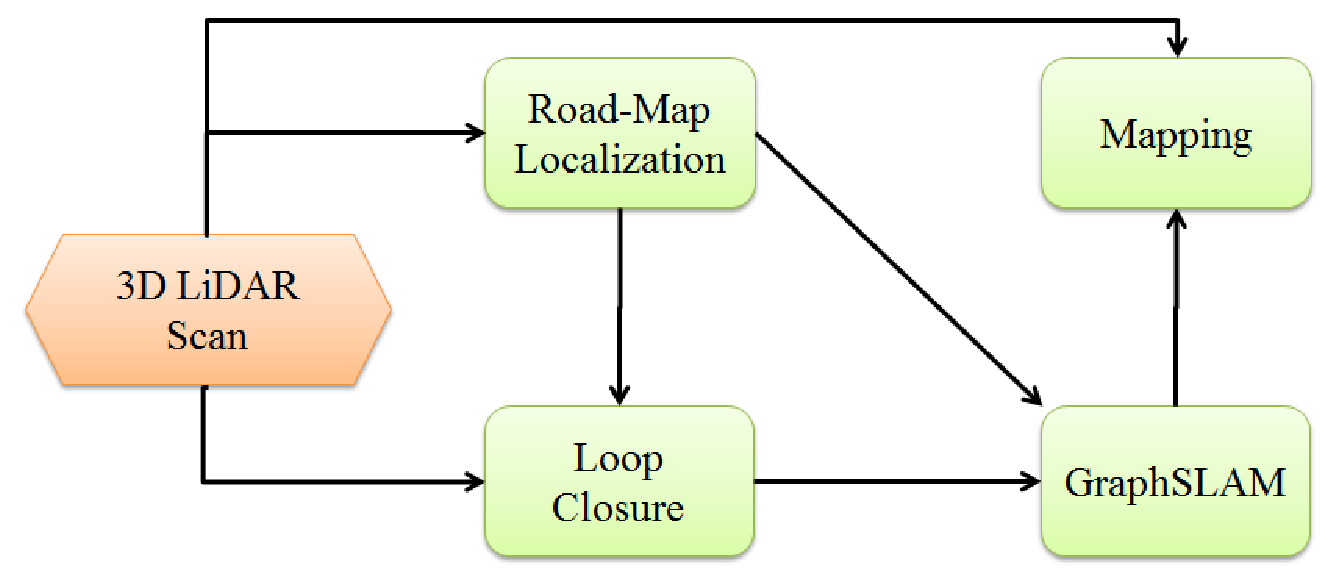
\includegraphics[width = 100 mm]{GraphSLAM.eps}
    \caption{Large-Scale Environment Mapping System (LEMS) Architecture. Firstly, a human drives IARA through the interest region and the sensor data are logged. Then, the Road-Map Localization system is executed to generate the Global Car Position and Visual-LiDAR Odometry. After that, the Loop Closure subsystem is used to detect revisited regions and to measure the displacement between the poses in the subsequent visits. Finally, the GraphSLAM subsystem is executed to estimate a feasible vehicle path and the Mapping subsystem is executed to build the environment grid map by projecting the velodyne point cloud from 3D to 2D, detecting obstacles, and placing them in the world using the GraphSLAM poses.}
    \label{Fig::FIGURE02}
\end{figure}

The Loop Closure subsystem receives as input the data from GCP and Velodyne point clouds, detects loop closure regions and estimates the displacement between the poses in the subsequent visits to the same region. The output of the loop closure subsystem, the data from Global car path and odometry are used to introduce restrictions to the GraphSLAM optimizer that is responsible for calculating the set of most likely poses given sensor data. Lastly, the mapping subsystem receives as input the Velodyne point clouds and the respective poses, calculated by the GraphSLAM, and outputs the environment occupancy grid map. It is important to note, however, that the proposed architecture can be easily extended to create any kind of grid map (e.g., re-emission grid maps, likelihood field grid maps, etc.).


\subsection{Loop Closure}

The loop closure subsystem has two objectives: firstly, to detect the poses of the robot when it revisits a region, and secondly, to measure the displacement of the poses in relation to the first visit caused by the dead-reckoning accumulated error.

To detect whether some region has already been visited, each GCP position data is compared with older GCP positions. If some old position has a smaller distance from the current GCP position than a pre-defined threshold (five meters, in this work) and the timestamp difference is bigger than a pre-defined threshold (in this work two minutes is used), a new loop closure is detected. In this case, both positions (the current one and the old one) are sent to the displacement measurement phase. If more than one position satisfies the loop closure condition, only the closest one is considered.

To estimate the displacement between two loop closure poses, we translate the Velodyne point clouds to the poses given by the GCP pose. Then, we register the point cloud of the second visit to the point cloud of the first visit using the GICP. This algorithm estimates the correction transformation that best fit a source point cloud to a target point cloud.

\subsection{GraphSLAM}

The GraphSLAM is a full-SLAM algorithm \cite{10thrun2006graph} in which the probabilistic variables are represented by graph vertices, and the sensor measurements are represented by graph edges. In this work, each vertex represents a robot pose (x-y and $\theta$) and edges correspond to sensor measurements and its uncertainties (represented as covariance matrices). Note that the GraphSLAM edges are the dead-reckoning, the loop closures and the GCP. Figure \ref{Fig::FIGURE03} illustrates an example of a graph.

\begin{figure}[ht]
    \centering
    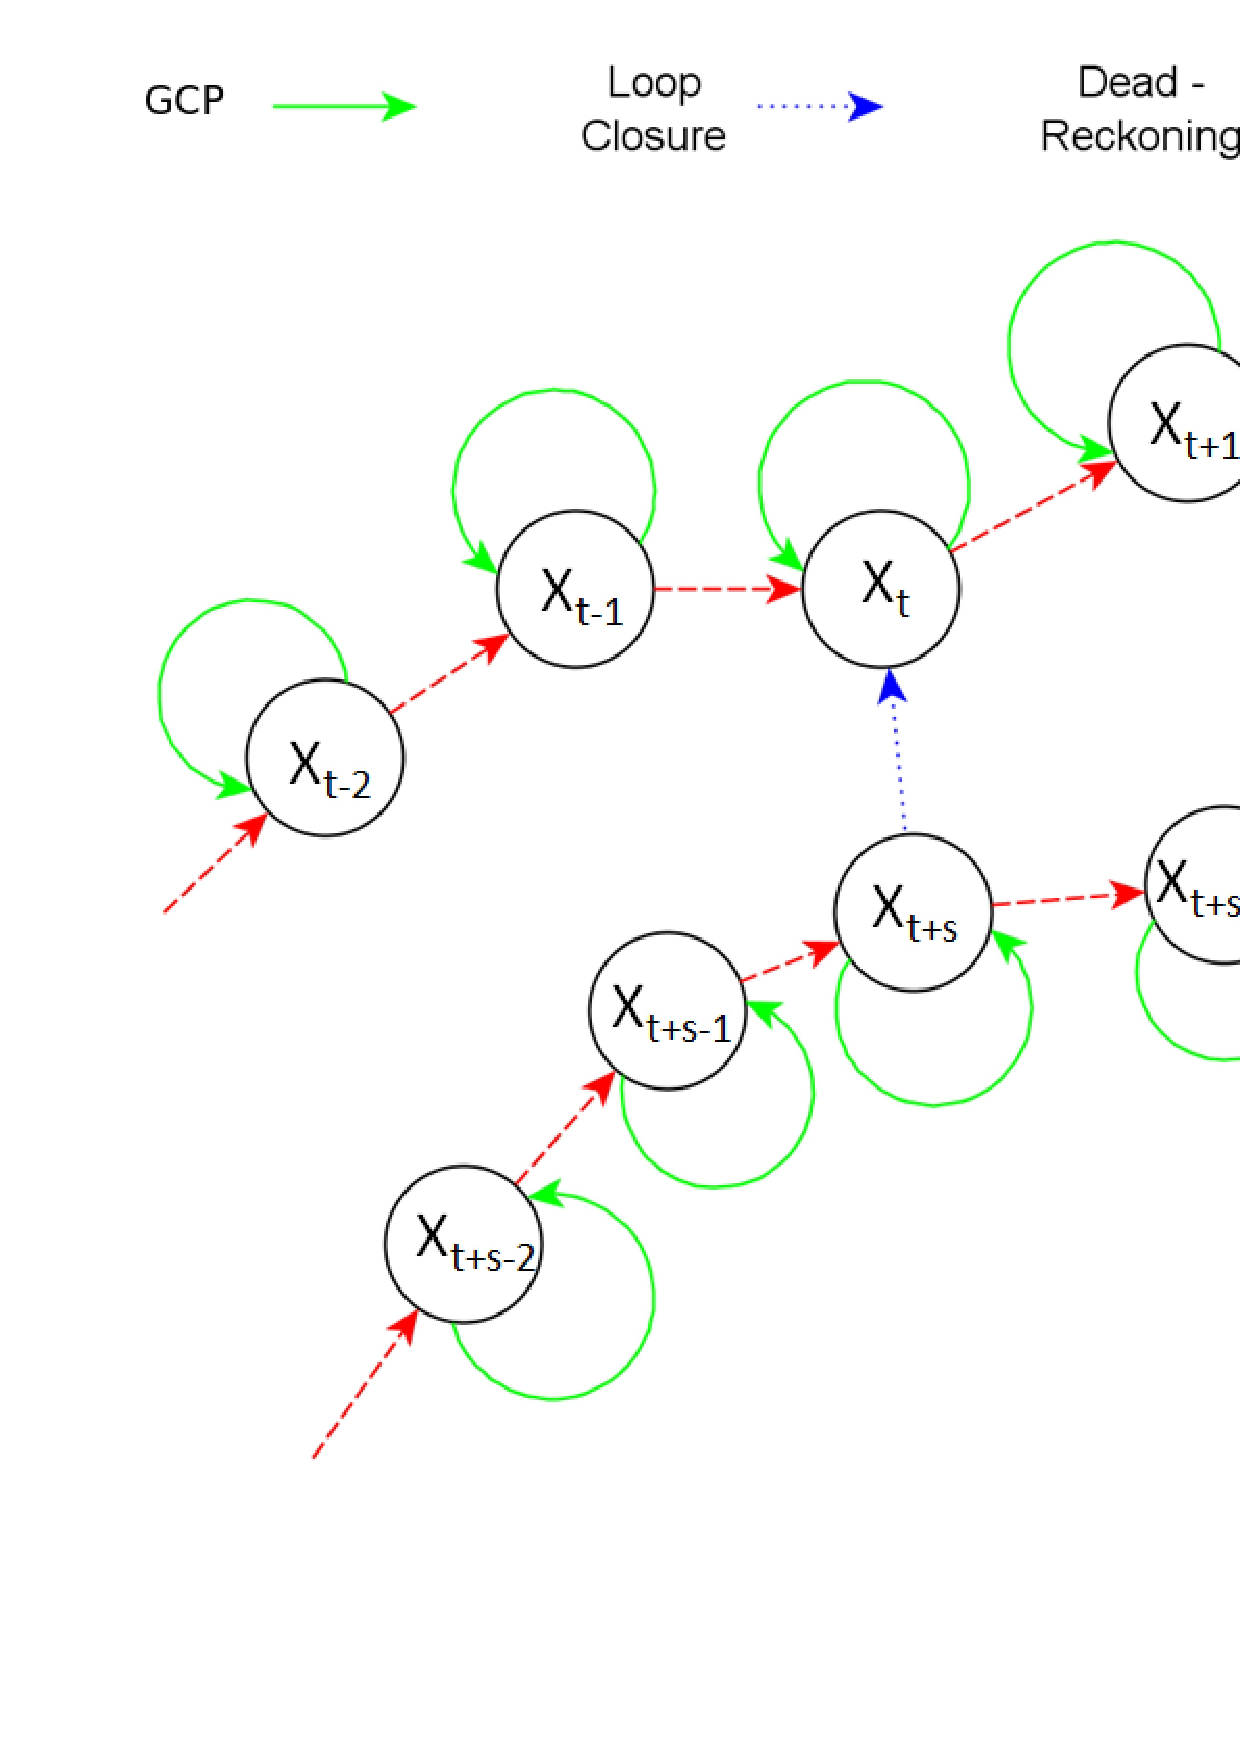
\includegraphics[width = 100 mm]{FIGURE03}
    \caption{Example of Graph Constructed by GraphSLAM. The black circles represent the poses, the red dashed edges represent the dead-reckoning displacements between two consecutive poses, the green filled unitary edges represent the GCP measurements, and the blue dotted edges represent the loop closures restrictions.}
    \label{Fig::FIGURE03}
\end{figure}

To estimate the most likely poses given the graph, several maximum-likelihood estimation techniques can be used. In special, when the sensor uncertainties are Gaussian, the maximum-likelihood estimation problem can be translated in a quadratic optimization problem solvable by gradient-based algorithms. The objective function of our GraphSLAM version is given by:
\begin{equation}
\label{Eq::GSLAMOBJ}
J=R_O+R_G+R_L
\end{equation}
where $R_O$ is the sum of odometry restrictions, $R_G$ is the sum of GCP restrictions, and $R_L$ is the sum of loop closure restrictions.

Because dead-reckoning and loop closure leads to Gaussian displacement restrictions and GCP lead to Gaussian global position restrictions, the log-likelihood objective function can be defined as:
\begin{equation}
\label{Eq::GSLAMlikelihoodOBJ}
\begin{array}{c}
J = \sum_{t}\left[ (X_t-(X_{t-1}+\delta_{t-1, t}))^TQ_t^{-1}(X_t-(X_{t-1}+\delta_{t-1, t}))\right]  \\
 + \sum_{t}\left[ (X_t-Y_t)^T R_t^{-1}(X_t-Y_t)\right]  \\
 + \sum_{X_A,X_B\in Loops}\left[ (X_B-(X_A+\delta_{X_A, X_B}))^TS_{X_A,X_B}^{-1}(X_B-(X_A+\delta_{X_A, X_B}))\right]
\end{array}
\end{equation}
where $X_t$ is a pose in time $t$,  $\delta_{t-1, t}$ is the estimated displacement between two consecutive poses $X_{t-1}$ and $X_t$ from dead-reckoning, $Y_t$ is a GCP measurement in time $t$, $\delta_{X_A, X_B}$ is a displacement from the pose $X_A$ to the pose $X_B$ (estimated by GICP) and $Q_t^{-1}$, $R_t^{-1}$ e $S_{X_A,X_B}^{-1}$ are the inverse covariance matrices from dead-reckoning, GCP and loop closure, respectively. During the optimization, the poses ($X_t$,$X_{t-1}$, $X_A$ and $X_B$) are changed and the sensors observations ($\delta_{t-1, t}$, $Y_t$ and $\delta_{X_A, X_B}$) and covariance matrices ($Q_t$, $R_t$ and $S_{X_A,X_B}$) stay fixed.


The mapping subsystem receives as input the Velodyne point clouds and its respective poses calculated by the GraphSLAM and outputs grid maps of the visited environment. The mapping used here is the same described in Section \ref{sec::ch2-mapping}. However, one important concern regarding mapping large-scale environments is the amount of memory used to store the map structure. A memory overflow can happen if the whole map is held in memory and the environment is sufficiently big. Taking this into account, we implemented a sub-map technique in which the mapped environment was divided in blocks of $50\times50$ meters, all of them with 0.2 meters of grid resolution (62,500 cells for each block). To reduce the memory consumption, the sub-map manager loads the blocks from the Hard Disk (HD) to the main memory in groups of nine blocks. It groups the small blocks to create a larger one with $150\times150$ meters. In addition, the sub-map manager is responsible for monitoring if the robot is in the central sub-map. When the robot crosses the central block boundaries, the sub-map manager loads new sub-maps to main memory and saves in HD and frees from memory the sub-maps that are not required anymore.

Figure \ref{Fig::FIGURE05} illustrates the procedure to switch sub-maps. The vehicle is initially located in the sub-map 4 (central block), and it begins to move in the direction of the sub-map 1 (Figure \ref{Fig::FIGURE05A}). Once the robot crosses the central sub-map boundary, three new sub-maps are loaded (9, 10 and 11) and incorporated into the sub-map held in memory (Figure \ref{Fig::FIGURE05B}). After that, the sub-map 1 becomes the new central sub-map and the sub-maps 6, 7 and 8 are saved in the Hard-Disk (HD) and freed from the main memory (Figure \ref{Fig::FIGURE05C}). Finally, the sub-maps are renamed as showed in Figure \ref{Fig::FIGURE05A}.

\begin{figure}[t]
\centering
\subfloat[]{
\begin{tabular}{|c|c|c|}
\hline
0 & 1 & 2 \\ \hline
3 & 4 & 5 \\ \hline
6 & 7 & 8 \\ \hline
\end{tabular}
\textbf{\label{Fig::FIGURE05A}}
}
\subfloat[]{
\begin{tabular}{|c|c|c|}
\hline
9 & 10 & 11 \\ \hline
0 & 1 & 2 \\ \hline
3 & 4 & 5 \\ \hline
6 & 7 & 8 \\ \hline
\end{tabular}
\label{Fig::FIGURE05B}
}
\subfloat[]{
\begin{tabular}{|c|c|c|}
\hline
9 & 10 & 11 \\ \hline
0 & 1 & 2 \\ \hline
3 & 4 & 5 \\ \hline
\end{tabular}
\label{Fig::FIGURE05C}
}
\caption{Illustration of the sub-map management technique. In all figures, each cell represents a $50\times50$ meter sub-map. The set of cells creates a $150\times150$ meters map that is used by the robot to localize itself and to navigate on the environment. At each instant, the robot "lives" only in the central sub-map. Whenever it crosses the boundary of the central sub-map, new sub-maps are loaded from HD to compose the new map in memory. Thereafter, the unnecessary sub-maps are saved on the disk and cleaned from the main memory. (a) $150\times150$ meters map that is kept on the main memory of the computer. (b) transition when the robot crosses the boundary of the central map and some of new sub-maps are loaded. (c) saving and freeing of the sub-maps that are no longer necessary.}
\label{Fig::FIGURE05}
\end{figure}

\section{Localization System}

The localization system developed in this work is a Particle Filter Localization (PFL) algorithm that processes the Visual-LiDAR Odometry to make predictions of the car movement. For the filter update, two different ways to compute the map-matching stage were implemented and evaluated in order to reduce the computational cost of the localization process and to increase the accuracy of the vehicle pose estimates. The first distance is an improvement of the Likelihood Field Map-Matching. The second is the Cosine between the a-priori grid-map (off-line map) and the local grid-map, both represented as vector entities.

\subsection {Online Map Construction}
Differently from the offline grid map ($m$), the local grid-map ($m_{local_{t}}$) is constructed on-the-fly by the techniques introduced in Section  \ref{sec::ch2-mapping}. It is an occupancy grid-map based on just one Velodyne twist scan at the time $t$, as shown in Figure \ref{Fig::OCU-ONE-SHOt}. As the map-matching distances do only consider the grid cells that represent obstacles in the local map, the set of selected grid cells is consequently very sparse. The local map is compacted by using the Compressed Row Storage (CRS) techniques \cite{bai2000templates}. 

The CRS stores the known cell values of the local map using three vectors, one vector for cell values, other for cell columns index, and the last one for the index in both other vectors (values and columns), where each line of the local map starts. In many cases this policy dramatically reduces (e.g. to just 3\%) the number of map queries for each particle. We consider as a map queries individuals access (reading) to the grid-cells during the process of the particle weight estimation. Figure \ref{Fig::VELODYNE-ONE-SHOT-MAP} shows the comparison between the number of point in one Velodyne twist scan (Figure \ref{Fig::POINT-CLOUD}) against the local map (Figure \ref{Fig::OCU-ONE-SHOt}). Consequently, the processing cost required in the map-matching stage is remarkably decreased. This stage is the most expensive operation in the process of localization using maps.

\begin{figure}[t]
\centering
    \subfloat[]{
\includegraphics[width=50mm]{Occupancy-oneshot.eps}
    \label{Fig::OCU-ONE-SHOt}}
    \subfloat[]{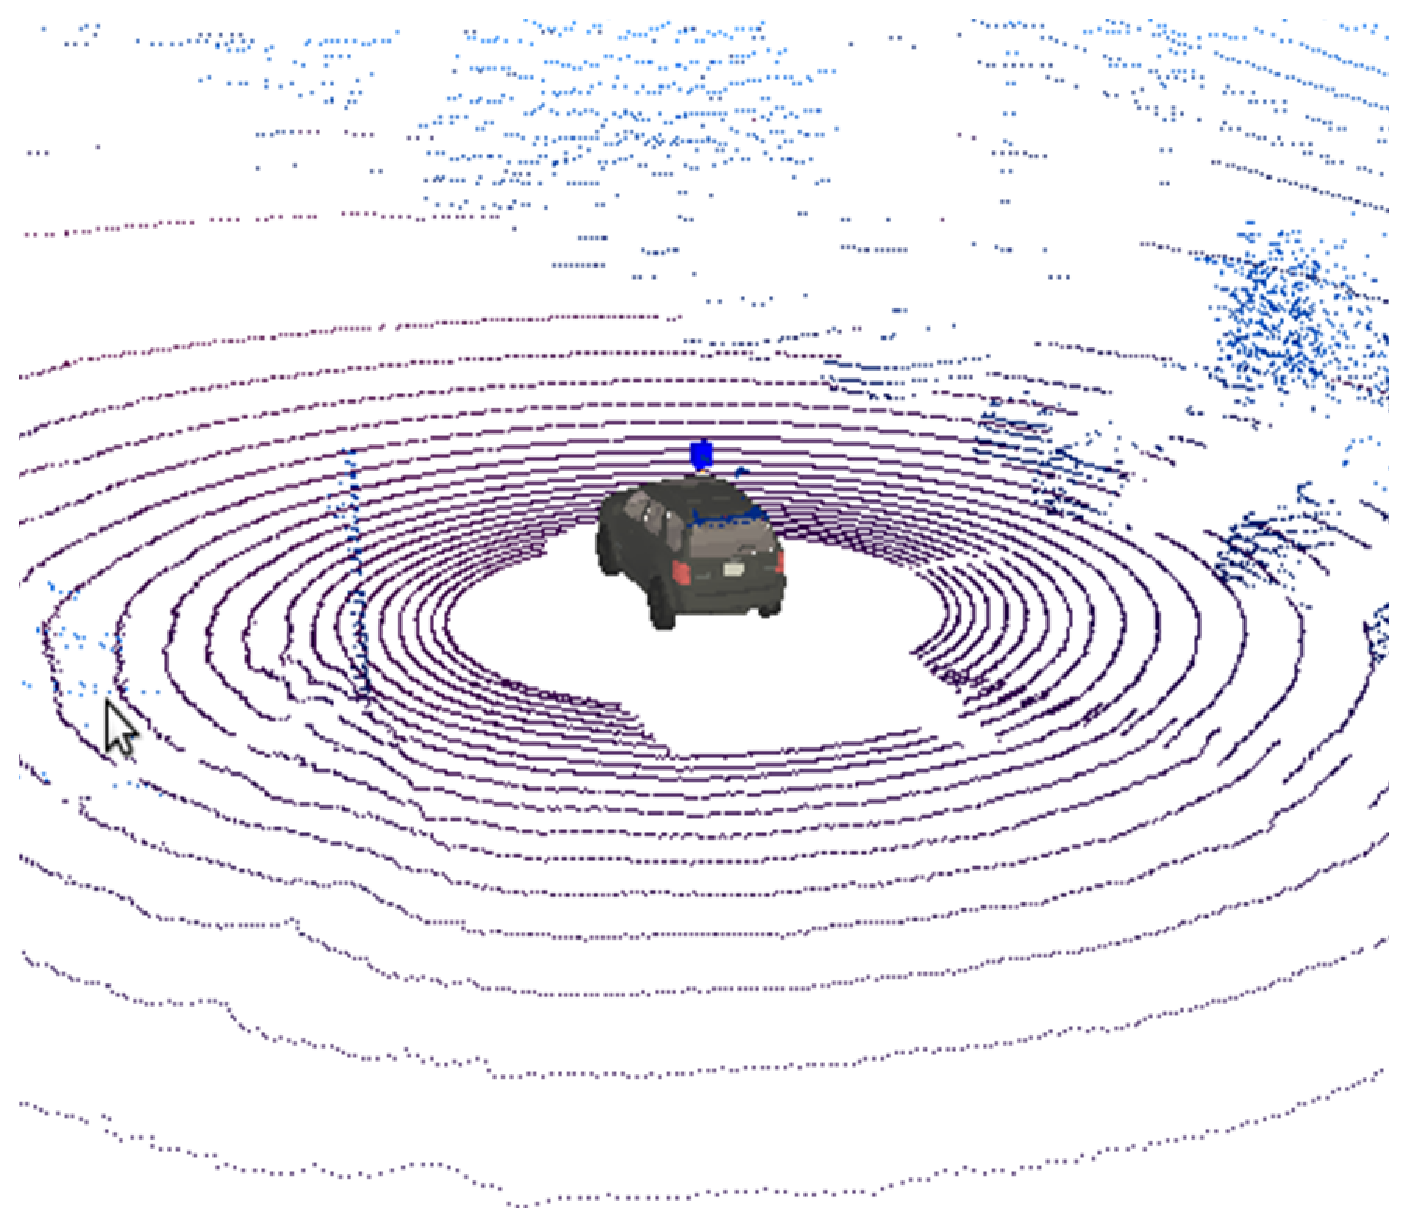
\includegraphics[width=60mm]{point-cloud.eps}
    \label{Fig::POINT-CLOUD}}
\caption{Local grid map based on measurements provided by a Velodyne 3D LiDAR sensor and projected to 2D (left). The black cells represent the obstacle identified in a Velodyne 3D imagery. The image illustrates part of a Velodyne point cloud in one spin (right). After mapping, the number of points that will be used to perform the map-matching was reduced severely.}
\label{Fig::VELODYNE-ONE-SHOT-MAP}
\end{figure}

\subsection{Particle Filter Localization}

The PFL is a probabilistic localization approach, which follows the recursive nonparametric Bayesian Filter, also known as Monte Carlo Localization \cite{26thrun2005probabilistic}. PFL represents the probability of the 3DoF pose $X=[x,y,\theta]$ (the position $x$ and $y$,and the orientation $\theta$) as a finite set of random particles. The set of particles is usually initialized by an uniform distribution over the workspace. Then, the filter runs iteratively, performing predictions about the robot movement and updates based on the measurements of the environment. For instance, after the initialization, the particles are sampled following the robot kinematic model using the odometry of the robot. This is usually called as prediction phase. When an exteroceptive measurement is available, an update step can be performed. In the update step, the generated local map is compared with the expected local map of each particle (based on the global offline map) in order to estimate the particles' weights. This phase is usually denominated the importance factor. Finally, the particles are drawn to select the most likely particles to compose the robot pose.

Generally, the PFL localizes the robot globally distributing the particles uniformly along the grid map $m$. Since the robot is running in outdoor places, in this work, the first position is selected manually as initial guess for the particles localization. Finally, the particles are sampled following a Gaussian distribution centered in the pose indicated and the covariance proportional (here, we are using 2 meters).
 
After its initialization step, the PFL runs iteratively in order to localize the vehicle using the provided a-priori map $m$. At each time step $t$, it predicts the vehicle motion, computes the particles weights and re-samples them. To estimate the vehicle motion from $t-1$ to $t$, the PFL uses the vehicle odometry data $u_t=\left\langle v_t,\omega_t\right\rangle $ ($v_t$ and $\omega_t$ are, respectively, the vehicle longitudinal and angular velocities) to generate a hypothetical vehicle motion. The estimation follows an Ackerman kinematic model that  moves a particle $k$ from the state $x_{t-1}^k$  to $x_t^k$ by adding Gaussian noise \cite{54sotelo2003lateral}. This phase involves sampling from the state transition distribution $p(x_t^k |u_t,x_{t-1}^k,m)$. The weight $w_t^k$ is computed for each particle $k$ by applying the map-matching distance between $m_{local_{t}}$ and m given $x_t^k$. The local map $m_{local_{t}}$  is aligned to grid map m given the pose of the robot in $m_{local_{t}}$ (central position) and $x_t^k$. At the end of each update step of the PFL algorithm, the particles are re-sampled to emphasize the most likely particles. The final estimation provided by the PFL to other client processes of the autonomous vehicle (such as the position controller) is the average of the values of the current particles population. 

\subsection{Log-Likelihood Map-Matching}

The high frequency localization proposed in this work computes the map-matching by summing the log of the likelihood in the Likelihood Field (LF) grid-map, specifically focusing on the grid cells that have a high probability of being an obstacle, in the local occupancy grid-map $m_{local_{t}}$. Eq.\ref{Eq::ch3-1} expresses the Log-Likelihood field distance estimation.
\begin{equation}
\label{Eq::ch3-1}
g(m_{local_{t}},x_t,m_{LF}) = \sum_{\forall(i,j)\in \Omega_t} \log(h(i,j,x_t,m_{LF}))
\end{equation}
where the subset $\Omega_t=\left\lbrace (i.j) \colon m_{local_{t}} (i,j)>0.5\right\rbrace $, i.e. cells which represent an obstacle. $m_{LF}$  is the Likelihood Field grid-map. $h(i,j,x_t,m_{LF})$  is a function that returns the value of a cell in the global grid map hit by a cell of the local map that was aligned (rotated and translated) given the hypothesis $x_t$. As a consequence of this policy, the number of map queries is remarkably reduced, making the full estimation process feasible to be performed in real-time. The weights for all the particles are evaluated based on the map matching instances, calculated for each of the particles. The particle weight $w_t^k$ for each particle $k$ is defined as follows:
\begin{equation}
\label{Eq::ch3-3}
w_t^k = \frac{\exp(g(m_{local_{t}},x_t^k,m_{LF}))}{\exp(\max_{i}(g(m_{local_{t}},x_t^i,m_{LF})))}
\end{equation}

\subsection{Cosine Map-Matching}

As an alternative to Log-Likelihood distance, we present the cosine distance to compute the map-matching. The Cosine between high dimension vectors has been used in Information Retrieval in order to measure the distance between two documents represented as vectors \cite{23baeza1999modern}. Due to its characteristics, the problem of map-matching is able to be treated in a similar way.

The Cosine distance evaluates the angular distance between two vectors in the $\Re^n$ space. In our approach, $n$ is the number of grid cells having $m_{local_{t}}(i,j)>0.5$. This measure evaluates the angular distance between know cells in $m_{local_{t}}$ and the corresponding cells in $m$. The Cosine distance is defined as follows:
\begin{equation}
\label{Eq::ch3-4}
cos(m_{local_{t}},x_t,m) = \frac{\sum_{\forall(i,j)\in \Omega_t} m_{local_{t}}(i,j) \cdotp h(i,j,x_t,m)}{\sqrt{\sum_{\forall(i,j)\in \Omega_t}m_{local_{t}}(i,j)^{2}}\sqrt{\sum_{\forall(i,j)\in \Omega_t}h(i,j,x_t,m)^{2}}}
\end{equation}
The Cosine distance varies between -1 and 1, where the lowest value represents the maximum dissimilarity and the highest one the maximum similarity. The negative values happen when most of the $m_{local_{t}}$ cells are aligned with unknown cells in $m$. This situation usually happens when a particle is placed in regions labeled to be unknown, or is placed close of them. To avoid such cases, the cosine is summed with one, $g(m_{local_{t}},x_t,m)=1+\cos(m_{local_{t}},x_t,m)$, and as a result the function output changes to $[0, 2]$. To compute the particles' weights, the function $g(\cdotp)$ is normalized. Then, the definition of the particles' weight is expressed according to the following expression:
\begin{equation}
\label{Eq::ch3-5}
w_t^k = \frac{g(m_{local_{t}},x_t^k,m) - \min_{i}(g(m_{local_{t}},x_t^i,m))}{\max_{i}(g(m_{local_{t}},x_t^i,m)) - \min_{i}(g(m_{local_{t}},x_t^i,m))}
\end{equation}


\chapter{Autonomous Cars Localization for GPS-denied Urban Environments}

\section{Introduction}


\section{Localization Based on Satellite Aerial Maps}

Figure 1 presents an overview of the proposed system architecture. Our system is divided into two main components: offline and online parts. The offline part is responsible for creating a large grey-scale map image of the region of interest. This is achieved by downloading individual aerial pictures and stitching them together.

The online part implements a Particle Filter Localization (PFL) algorithm [15]. The PFL system is initialized by sampling the particles on top of the aerial image map according to the first GPS and compass readings. During the prediction phase, the PFL considers the vehicle's movement disturbed by a Gaussian noise to cover the real positions as hypotheses. Thereafter, the LiDAR is used to create a local re-emission map, which is built using the infrared reflectance of the Velodyne's lasers together with the returned distance information and dead-reckoning. This re-emission map is accumulated for a few time steps and it is compared against the aerial map in order to estimate the particles' weights. The comparison is performed using NMI. Based on the weights, the best particles are selected to calculate the global pose according to the weighted average of their position. Please note that the information from the GPS and the compass are used only to globally initialize the PFL algorithm.

\subsection{Offiline Aerial Map}

A large aerial image for the region of interest is created by first downloading individual images with a $640\times640$ pixel resolution. Individual images overlap each other and the overlapping region is used to calculate the correspondences between them that are necessary for image registration and stitching. This step is performed once manually using the Microsoft ICE software. Unfortunately, the minimum grid-size (zoom level) of the region of interest is close to 0.29 meters. In order to avoid rounding problems, we rescaled the stitched map to 0.2 meters. Figure \ref{Fig::Path} shows the car's route and aerial images of challenging environments where the car was driven and localized (red line).

\begin{figure}[ht]
    \centering
    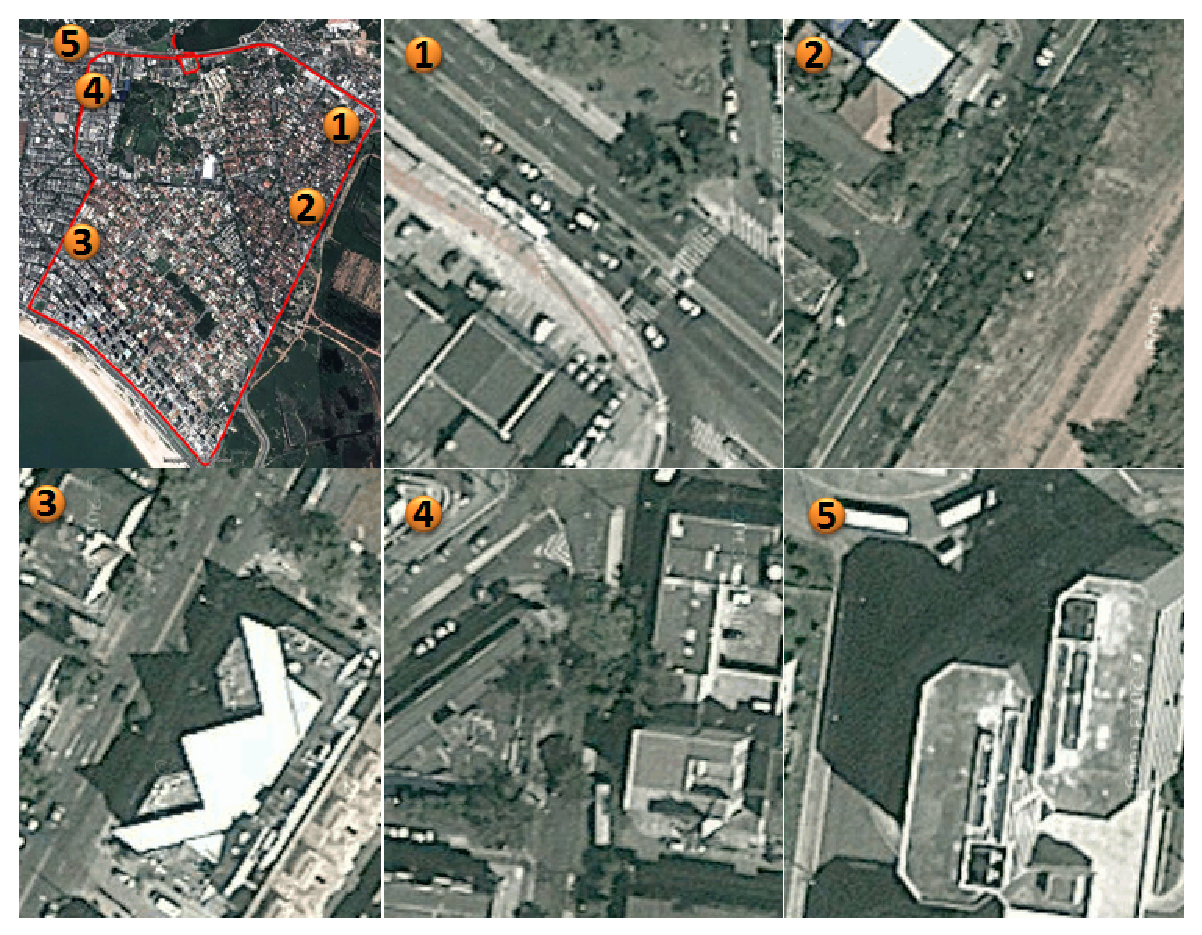
\includegraphics[width = 100 mm]{path.eps}
    \caption{Satellite map images used to localize the robot in a large urban area. The red line on the top-left image represents the car's route. The other images (1-5) are zoom up examples of aerial image maps used by our approach to localize the vehicle.}
    \label{Fig::Path}
\end{figure}

\subsection{Online Re-emission Grid-Map}

An online short-term re-emission grid-map (a local top view image) is built with $60\times60$ meters and 0.2 meters of resolution per pixel. This grid-map is a gray-scale image (i.e., $[0, 255]$) produced by the projection of every laser in 2D (see Figure \ref{Fig::Remission1}). Every pixel, i.e. map cell, in the grid-map stores the average of the infrared reflectance of the rays which touched it. The map shows several features (such as curbs, lanes, sidewalks, asphalt, etc), which are important for feature-comparison in the localization process of the mobile robot. Note that the short-term map accumulates the information of several Velodyne's scans in an area of approximately 3600 $m^2$ and that the robot dead-reckoning is considered when posing the scans in the local map. Figure \ref{Fig::Remission1} shows the short-term map after some Velodyne's scans. In this figure, the blue parts are non-sensed areas in the environment, gray scale areas are the average of the infrared reflectance, and the orange rectangle illustrates the robot position. Note that non-sensed areas (i.e. blue areas) are not considered during the distance measurement computation.



\begin{figure}[ht]
    \centering
    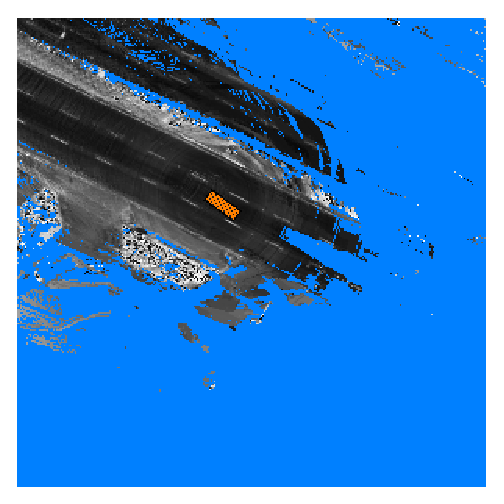
\includegraphics[width = 50 mm]{Remission1.eps}
    \caption{Local short-term re-emission grid-map with $60\times60$ meters built using the LiDAR. In this figure the blue parts are the non-sensed areas in the environment. Grey values indicate the average values of the laser infrared reflectance. The orange rectangle illustrates the robot position given by the dead-reckoning.}
    \label{Fig::Remission1}
\end{figure}

\subsection{Grid Map Construction and Representation}
\label{sec::ch2-mapping}

The mapping subsystem receives as input the Velodyne point clouds and its respective poses calculated by the dead-reckoning and outputs local grid maps.  In the grid maps, the environment is divided into cells with the same size (the size of the cells is usually called map resolution) and each of these cells contains some kind of local information about the environment.  There are several types of grid maps, e.g. occupancy grid maps, re-emission grid maps and likelihood-field grid maps. In occupancy grid maps, each cell contains the probability of the cell being occupied by an obstacle. In re-emission grid maps, each cell stores the average infrared reflectance of the rays that hit that cell \cite{13levinson2007map}.Thus, re-emission grid maps have the appearance of an image of the ground plane. Finally, in likelihood-field grid maps, each cell stores the Gaussian of the distance to the nearest obstacle \cite{26thrun2005probabilistic}.

To illustrate the described maps, \ref{Fig::FIGURE04A}, Figure \ref{Fig::FIGURE04B}, and Figure \ref{Fig::FIGURE04C} show occupancy grid map, re-emission grid map and likelihood-field grid map. All the maps have $60\times60$ meters and $0.2$ meters of map resolution. In Figure \ref{Fig::FIGURE04A}, the occupancy probability is represented in gray-scale where $255$ is the minimum probability of obstacles and $0$ is the maximum probability. The blue areas are unknown places in the environment. In Figure \ref{Fig::FIGURE04B}, the re-emission of the cells hit by the sensor rays are shown in gray and the blue area represents not hit cells. In Figure \ref{Fig::FIGURE04C}, the occupancy likelihood field is represented in gray-scale, where $255$ represents the lowest occupancy likelihood and $0$ represents the highest occupancy likelihood. The likelihood field model is an ``ad hoc'' alternative to the traditional beam model. While it lacks a plausible physical explanation, it provides important advantages, such as smoother posteriors even in cluttered spaces, and more efficient computation \cite{26thrun2005probabilistic}. In the likelihood field model, the probability of a sensor measurement is obtained by measuring the distance from the laser reading to the nearest obstacle in the map and applying this distance to a zero-centered Gaussian \cite{26thrun2005probabilistic}. Naturally, the probability is maximal when the distance is zero (the laser reading hit an obstacle in the map), and decreases as the distance get bigger. Because of this feature, areas of the map in which there are no information about obstacles (and it includes unseen areas), are filled with close to zero occupancy probabilities once their distance to the nearest obstacle are significantly bigger than zero. Even we emphasizing the development of occupancy grid maps, the LEMS can be adapted, with small modifications, to generate likelihood field-based (or any other kind of) grid maps.

\begin{figure}[t]
	\centering
	\subfloat[]{
\includegraphics[width=42mm]{Occupancy1}
		\label{Fig::FIGURE04A}}
	\subfloat[]{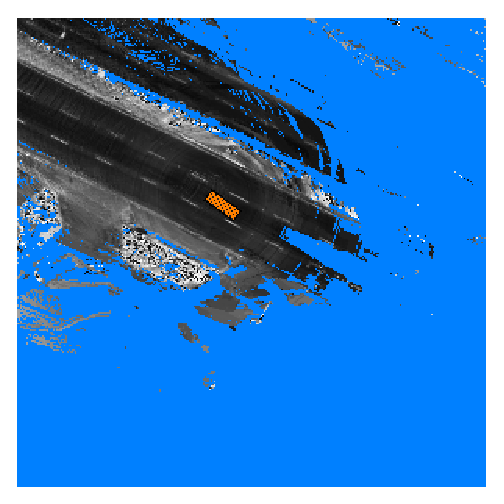
\includegraphics[width=42mm]{Remission1}
		\label{Fig::FIGURE04B}}\\
	\subfloat[]{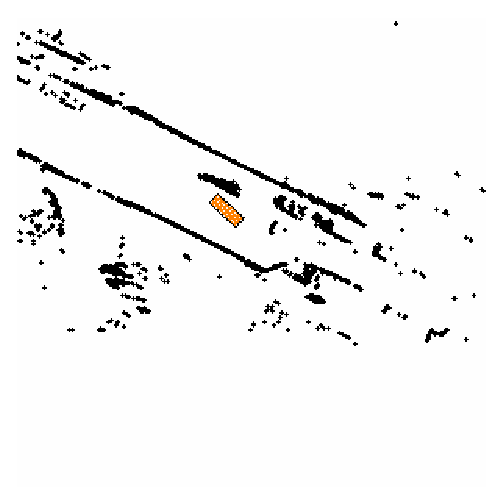
\includegraphics[width=42mm]{Occupancy3}
		\label{Fig::FIGURE04C}}
	\caption{Maps constructed by the Mapping process. (a) Occupancy grid map with $60\times60$ meters and 0.2 meters of resolution built using 3D LiDAR sensor projected to 2D. The blue parts are unknown places in the environment. (b) Re-emission grid map. (b) Likelihood-Field grid map.}
	\label{Fig::FIGURE04}
\end{figure}

The algorithm to build occupancy grid maps consists of initializing all cells with a neutral probability and then increasing or decreasing the cell occupancy probability depending if the laser ray hits an obstacle or a free area. The classical choices for the neutral probability are to use $0.5$ to represent that a cell has the same probability of being occupied or free, and to use an invalid value (e.g. $-1$) to represent that the cell occupancy probability is unknown. In this work, we used the second option. To avoid numerical inconsistency due to near to one or near to zero probabilities, we represent the occupancy probability using log-odds \cite{26thrun2005probabilistic}.

The data provided by the Velodyne sensor was used to update the occupancy probability of the map cells. The Velodyne consists of a set of vertical lasers that spins around the vertical axis in order to capture a 3D point cloud of the environment. As Velodyne provides point clouds in 3D spherical coordinates, it is necessary to project the rays to 2D to calculate the cells hit by the rays. Due to the particular structure of the sensor readings, we used a special method to detect if a laser ray hits an obstacle or a free area (the method is described in detail in the next subsection). Besides of updating the cells hit by the laser rays, we used a ray cast scheme to quickly mark the free areas close to the vehicle. This scheme consists of decreasing, for each set of vertical readings, the occupancy probability of the grid cells between the sensor and nearest detected obstacle.

\subsection{Obstacle Classification}

Here, we describe how to detect if a Velodyne ray hits an obstacle or a free area. Our obstacle detection technique assumes that the 3D point clouds are represented in spherical coordinates. We will use the notation $z_t^{i,j}$ to represent the $i^{th}$ ray of the $j^{th}$ vertical set of readings captured at instant t. To compute the obstacle evidence (OE) of the ray $z_t^{i+1,j}$, its size projected on the ground is compared with the size of the previous ray $z_t^{i,j}$ projected on the ground as well. If there are no obstacles on the road, the measured difference (MD) between the sizes of the rays will be equal to an expected distance (ED). On the other hand, if there are obstacles, the difference between the rays sizes projected on the ground will be less than the expected difference (see an illustration at Figure \ref{Fig::FIGURE06}).  With this, the obstacle evidence can be calculated by:
\begin{equation}
\label{Eq::ObstacleEvidence}
OE\left( z_t^{i+1,j}\right) =\frac{ED \left( z_t^{i,j},z_t^{i+1,j}\right) -MD\left( z_t^{i,j},z_t^{i+1,j}\right) }{ED\left( z_t^{i,j},z_t^{i+1,j}\right) }
\end{equation}
where $MD(.)$ is the measured difference and $ED(.)$ is the expected difference between two consecutive vertical rays' sizes projected on the ground.

\begin{figure}[ht]
	\centering
	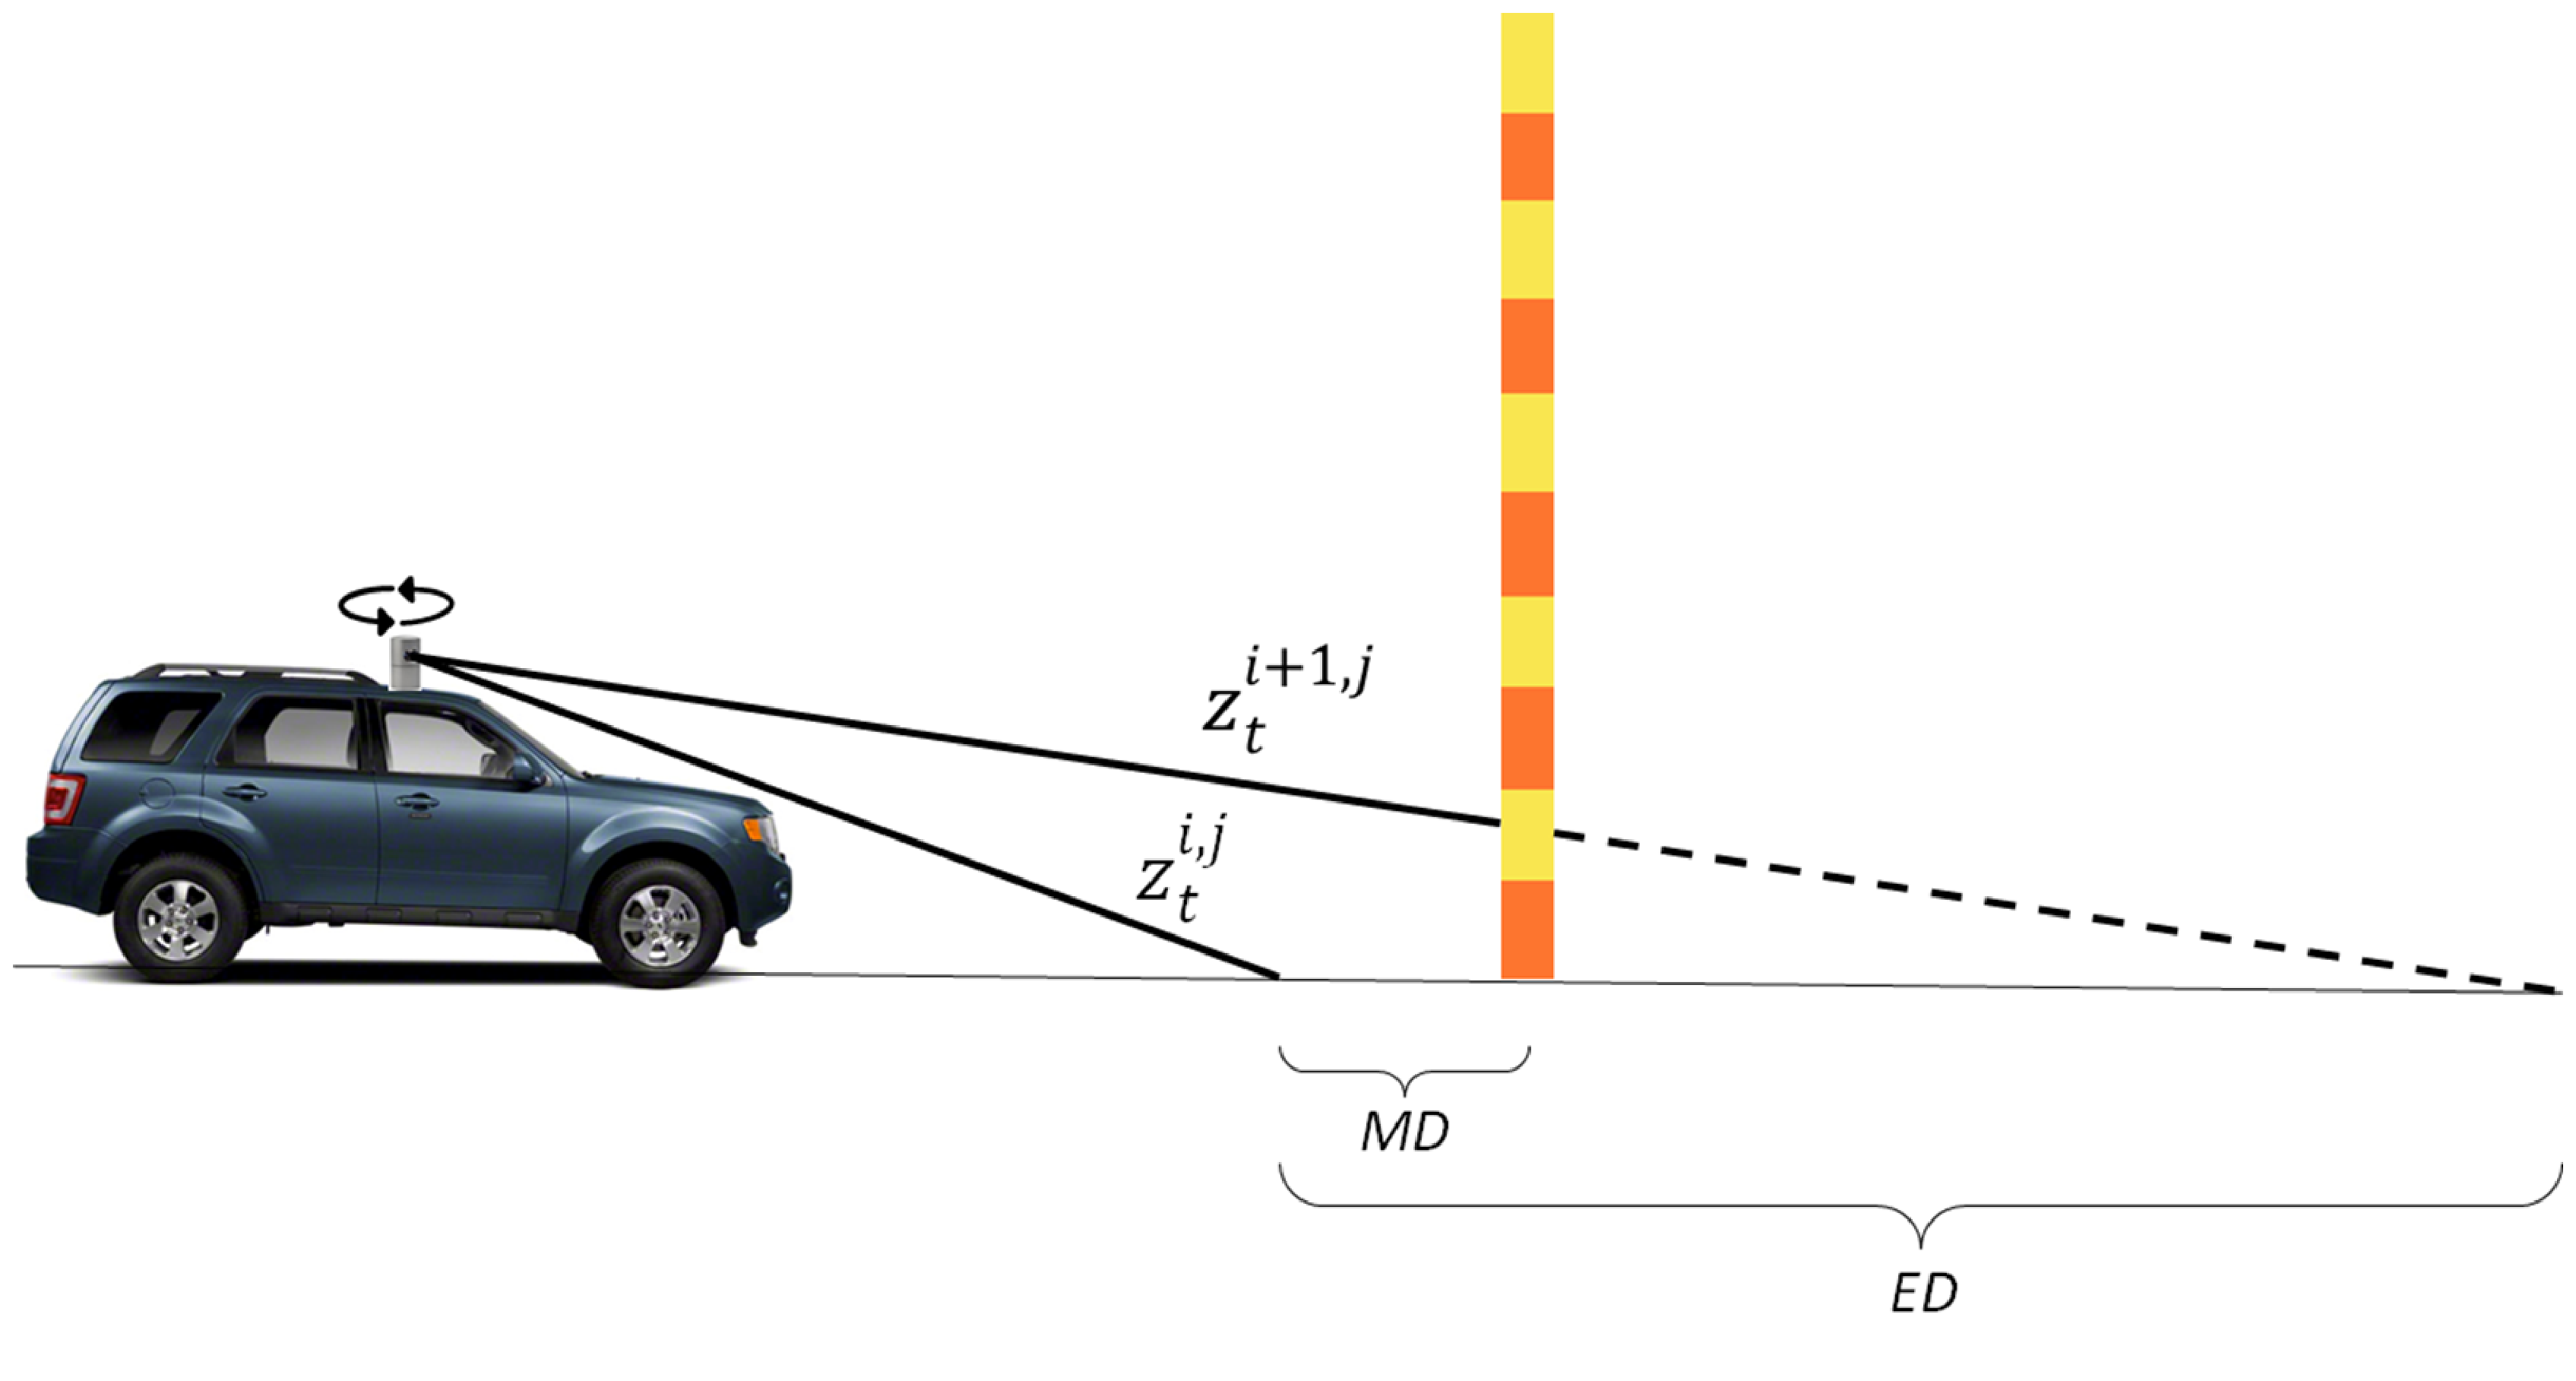
\includegraphics[width = 100 mm]{FIGURE06}
	\caption{Illustration of the obstacle detection scheme. Firstly, two consecutive Velodyne rays are projected on the ground. Then, the difference between the expected and the measured rays sizes on the ground are used to estimate the obstacle evidence.}
	\label{Fig::FIGURE06}
\end{figure}

The $MD(.)$ value is computed projecting two consecutive vertical rays on the ground and subtracting them:
\begin{equation}
\label{Eq::MeasuredDifference}
MD\left( z_t^{i,j},z_t^{i+1,j}\right) =\left| Pr\left( z_t^{i,j}\right) -Pr\left( z_t^{i+1,j}\right) \right|
\end{equation}
where  $Pr(.)$ is a ground projection function.

The expected difference value $ED(.)$ is calculated using a geometrical model of two vertical rays hitting the ground in an obstacle free environment. This geometrical model is illustrated in Figure \ref{Fig::FIGURE07}. In this Figure, $h$ represents the sensor height relative to the ground, $\alpha$ and $\beta$ are the vertical angles of ray $z_t^{i,j}$ and ray $z_t^{i+1,j}$, $b=Pr\left( z_t^{i,j}\right) $, $a=Pr\left( z_t^{i+1,j}\right) $, and $r$ is the length of the ray $Pr\left( z_t^{i+1,j}\right) $. The angles $\omega$ and $\gamma$ are auxiliary variables used in the $ED$ computation.

\begin{figure}[ht]
	\centering
	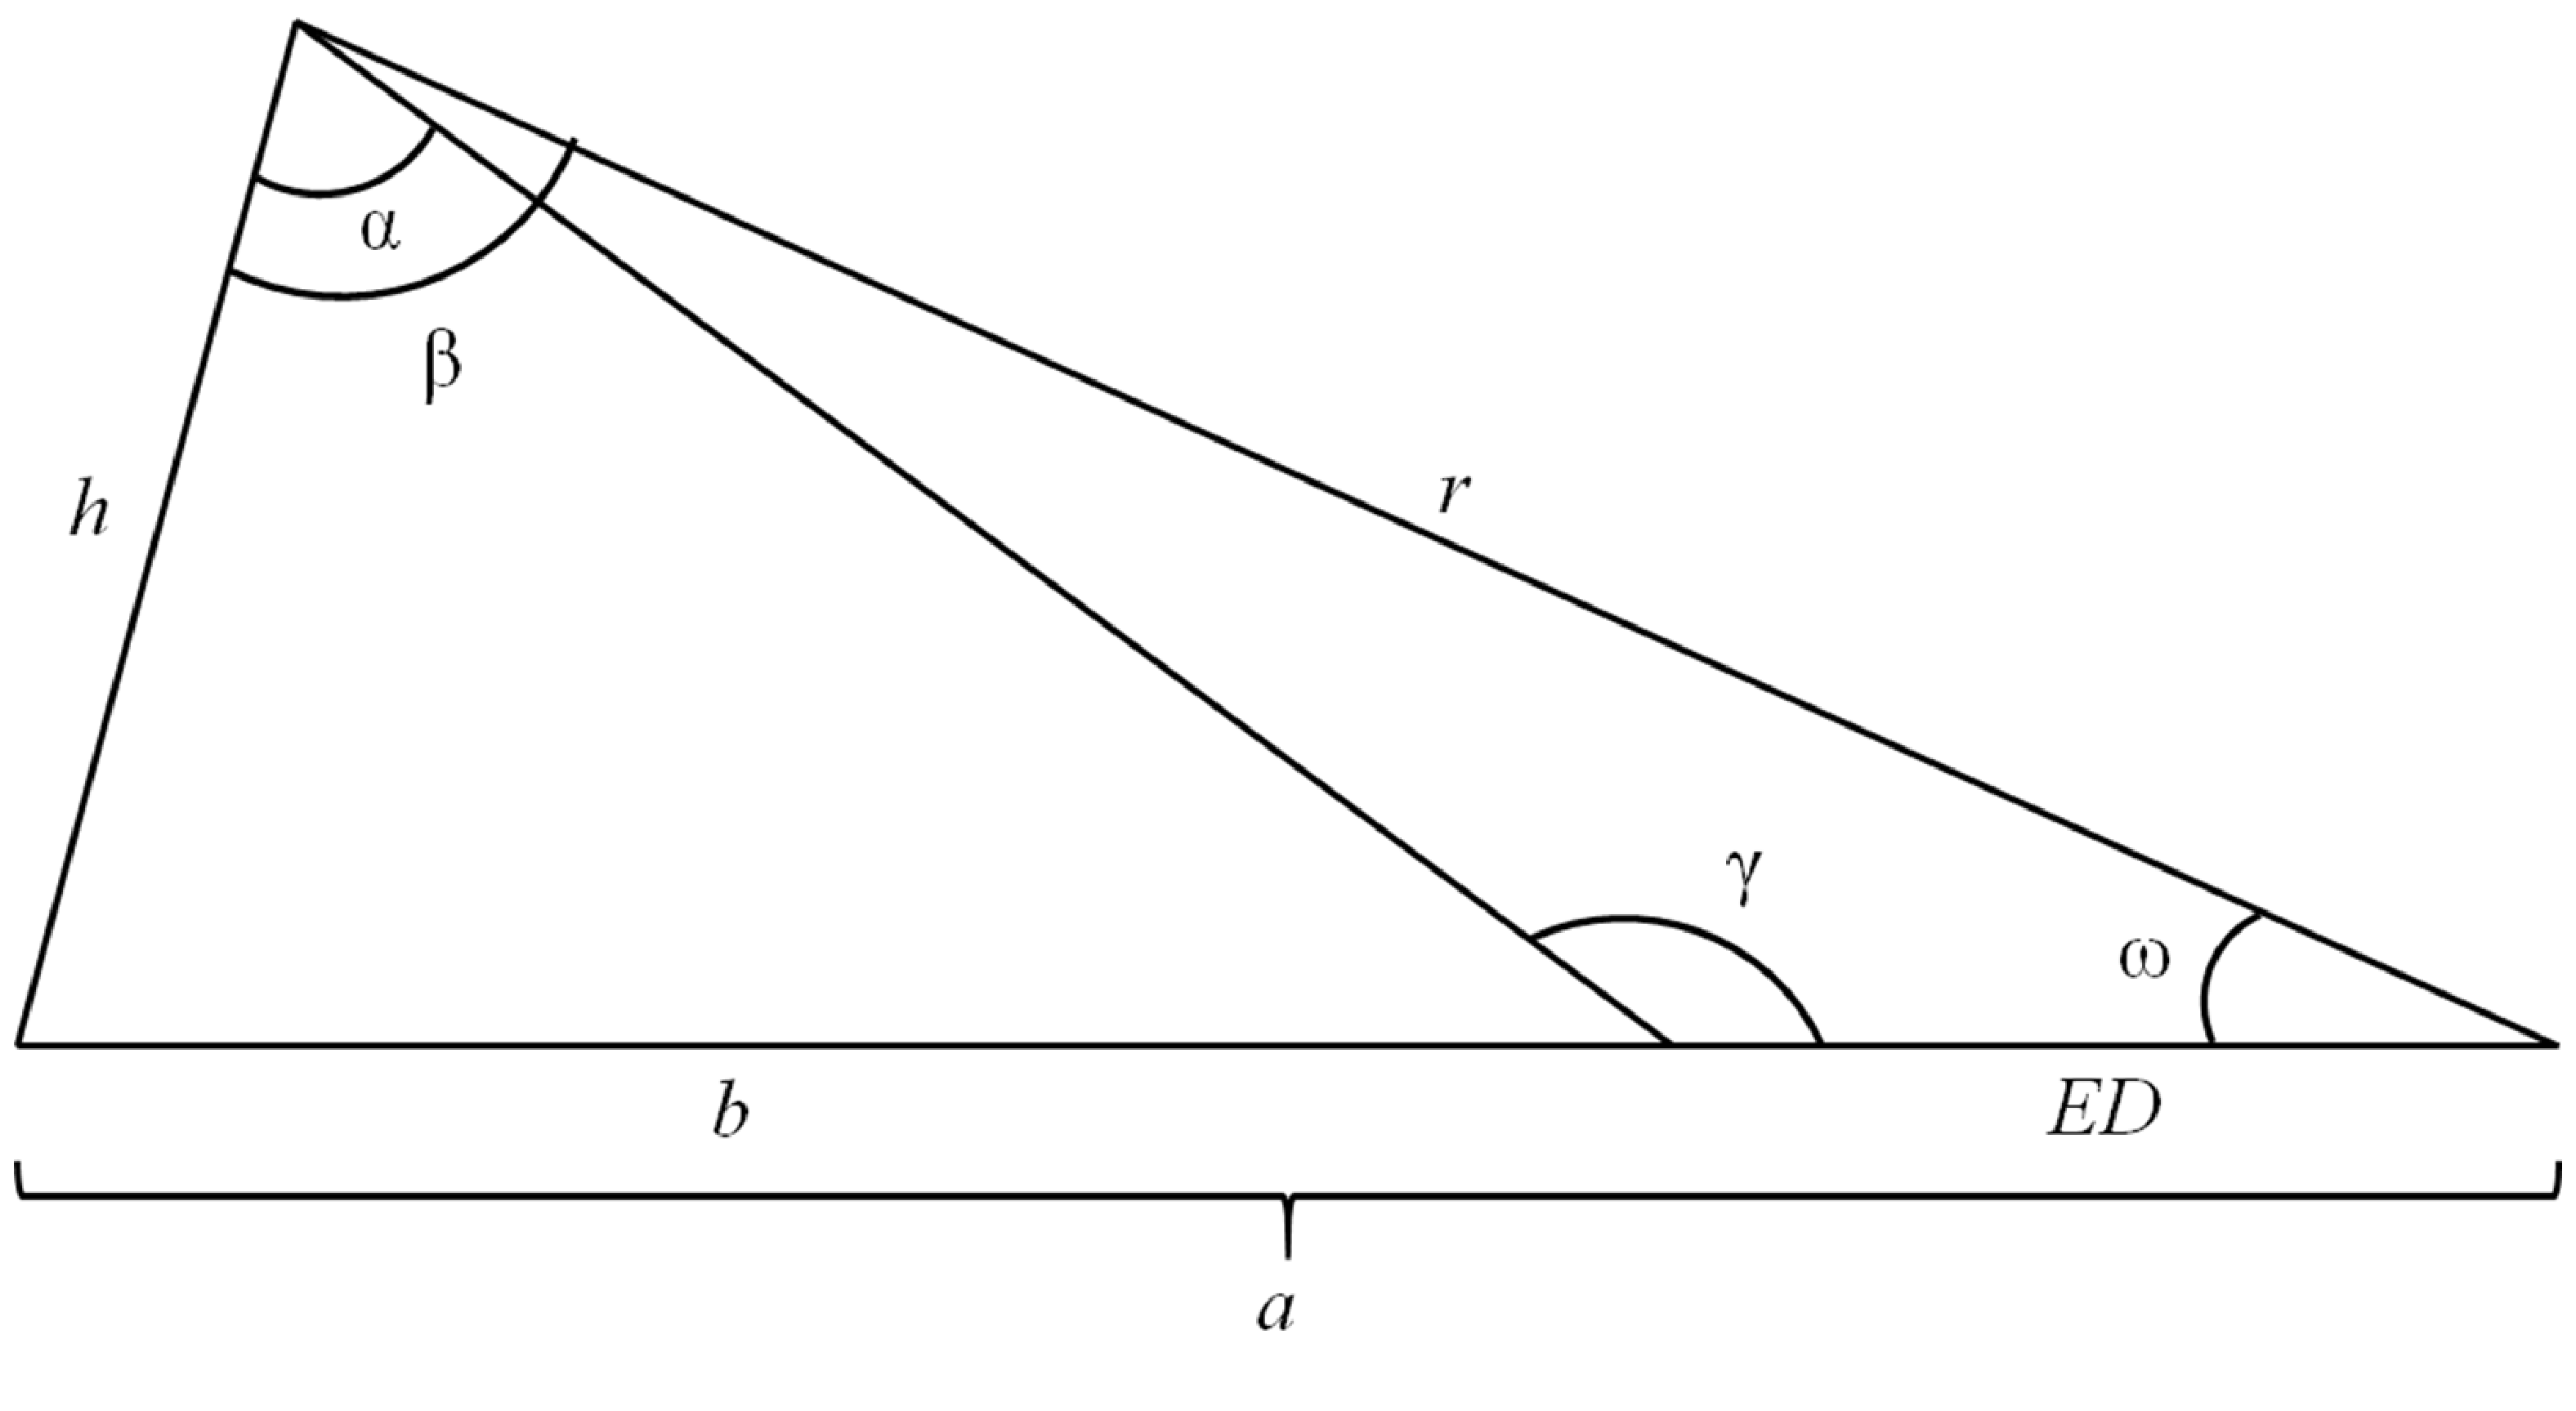
\includegraphics[width = 100 mm]{FIGURE07}
	\caption{Geometrical Model used to compute the expected value between two vertical 3D LiDAR rays projected on the ground.}
	\label{Fig::FIGURE07}
\end{figure}

The first step to compute $ED\left( z_t^{i,j},z_t^{i+1,j}\right) $ is to apply the sine law as follows:
\begin{equation}
\label{Eq::10}
\frac{\sin(\gamma)}{r}=\frac{\sin(\beta-\alpha)}{ED\left( z_t^{i,j},z_t^{i+1,j}\right)}
\end{equation}
and
\begin{equation}
\label{Eq::11}
ED\left( z_t^{i,j},z_t^{i+1,j}\right) = \frac{r\sin(\beta-\alpha)}{\sin(\gamma)}
\end{equation}
Then, the angle $\gamma$ can be computed by:
\begin{equation}
\label{Eq::12}
\gamma = \pi - \omega -(\beta-\alpha)
\end{equation}
The angle $\omega$ can be calculated by:
\begin{equation}
\label{Eq::13}
\frac{\sin(\beta)}{a}=\frac{\sin(\omega)}{h}
\end{equation}
and
\begin{equation}
\label{Eq::14}
\omega = \arcsin \left( \frac{h\sin(\beta)}{a} \right)
\end{equation}
After that, $a$ can be calculated using the cosine law:
\begin{equation}
\label{Eq::15}
a = \sqrt{h^2+r^2-2hr\cos(\beta)}
\end{equation}

Replacing the Equation \ref{Eq::15} in \ref{Eq::14}, \ref{Eq::14} in \ref{Eq::12} and \ref{Eq::12} in \ref{Eq::11}, the expected distance between two consecutive 3D LiDAR rays is given by:
\begin{equation}
\label{Eq::16}
ED\left( z_t^{i,j},z_t^{i+1,j}\right) = \frac{r\sin(\beta-\alpha)}{\sin \left( \pi -(\beta-\alpha) - \arcsin \left( \frac{h\sin(\beta)}{\sqrt{h^2+r^2-2hr\cos(\beta)}} \right) \right)}
\end{equation}

After computing the obstacles evidence $OE$, the occupancy probability $PO$ is given by:
\begin{equation}
\label{Eq::17}
PO = \frac{1}{\sqrt{2\pi\sigma_{OD}^2}}\exp \left( \frac{-OE\left( z_t^{i+1,j} \right)^2}{2\sigma_{OD}^2} \right)
\end{equation}
where $\sigma_{OD}$ is the obstacle detection standard deviation. The value was found during empirical experimental tests (in this work, we used $0.8$).


\subsection{Dead-Reckoning based on Scan-Matching}

The dead-reckoning is an important part of our system that detects intersection. It is used to place the Velodyne scan in the local map during the mapping. Mistakes to pose these scans can generate errors in the placement of the rays on the map. These problems in general happen because the car odometer may have bias, pour measurement and wheel slips. 
%If the car kinematic model is based on the steering model, to estimate the car steering-wheel bias can be a hard task, since inclinations on the ground would affect the calibration in different scenarios. This way, an alternative for having better pose estimation by the dead-reckoning is applying the gyros model instead
In normal condition (without rain), the slips does not affect so much the dead-reckoning in asphalt roads. But, in different sort of terrain such as grass, rocks, and soil, which has different friction coefficient, the slips are unpredictable and if they are wet it becomes worse. Alternatively, the ground type could be detected by processing the camera installed on-board, but the light condition limited its application. Note, this slips estimation is very important for vehicles that operate in mines, farms, desert or off-road since the ground is frictionless \cite{woodsterrain}.

Therefore, a scan matching has been applied between two Velodyne's point clouds in order to estimate the dead-reckoning. I.e., this system computes the car odometries (car speed and angular velocities) using only Velodyne imageries. It is well known as Visual-LiDAR Odometry \cite{Zhang_LOAM, Zhang_V-LOAM, zhang2014real}. It begins with the car stationary registering the scans, whenever the car starts to move the difference between the pose will be used to calculate the odometries, with them predictions of the car movement will be computed to generate initial guesses for later scan-matches.

Another fact, The Velodyne HDL32-E spins 20 times per second scanning with 32 laser shots that take 46.09 $\mu$sec, so, for each $360^{o}$ scan, the Velodyne takes 50 msec. If the car speed is about 10 m/s, the car will travel around 0.5 meter to complete one full $360^{o}$ scan. This way, if the car speed and turn are not considered to pose every 32 laser shots in the right place, the same static objects in consecutive revolution is going to be in different places in the world. Consequently, the quality of the matching will degrade.

In this works, the Generalized-ICP (GICP) has been applied to provided the matches. We considered the GICP to perform point cloud registration since it was designed to work with Velodyne points \cite{58segal2009generalized}. Usually, the GICP has problems to work on-line using dense point clouds as the Velodyne one. Thus, using a the whole points of the spins, the time to process one frame is over 0.5 seconds. To reduce the computational time, a 3D voxel-grid operation has been employed with a grid-size of 0.6 meters. Now, it may register 10 frames per second.  Figure \ref {Fig::Dead_reckoning} shows Visual-Lidar Odometry path (dead-reckoning) (green) compared against to the GPS (red).

\begin{figure}[ht]
	\centering
	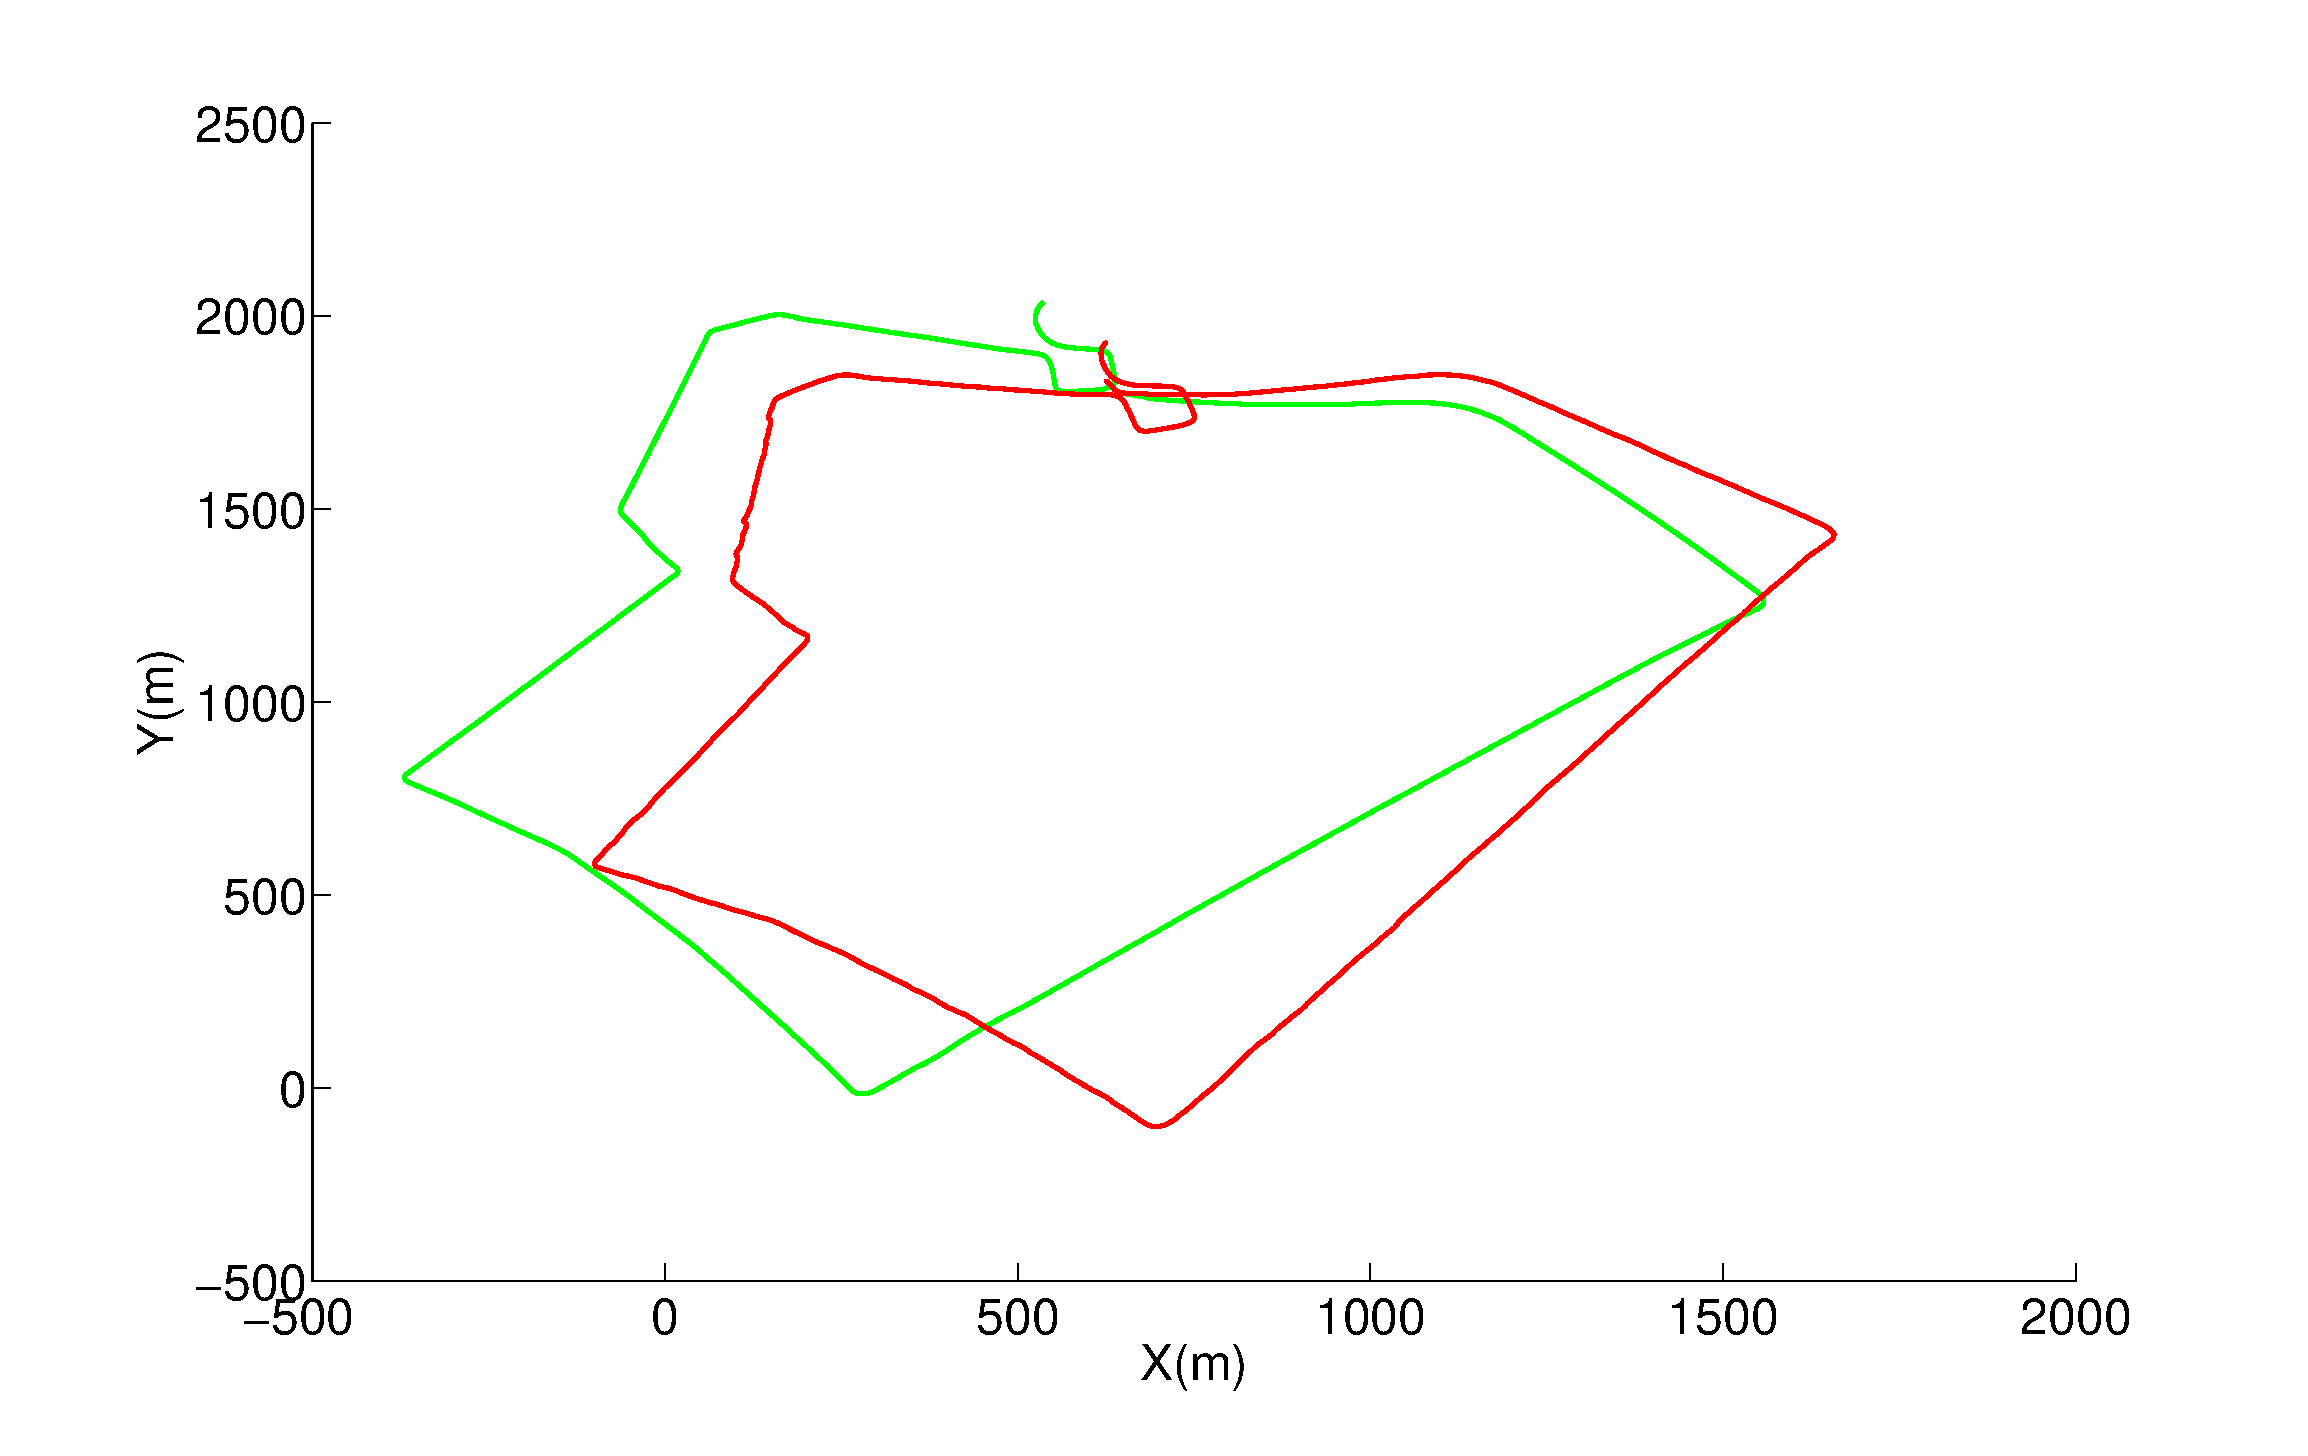
\includegraphics[width = 150 mm]{Dead_reckoning.eps}
	\caption{The car dead-reckoning estimated by the Visual-Lidar Odometry. The green and red lines represent the dead-reckoning and GPS respectively.}
	\label{Fig::Dead_reckoning}
\end{figure}



\subsection{Normalized Mutual Information}

The Normalized Mutual Information (NMI) is a variant of Mutual Information that has the capacity for measuring different types of relationships between variables [14]. NMI has been used to measure the relation between images captured from different sources. For instance, this probabilistic distance is widely used in medical image registration, where the pictures are taken from different devices with dissimilar color spectrum [18]–[20]. 

Because the aerial image map and the re-emission map also originate from devices with different image construction principles, in this work, the NMI metric is used to measure the distance between an aerial image map ($m$) and a re-emission local map ($m_{local}$). The NMI distance is defined as follow:
\begin{equation}
\label{Eq::NMI}
NMI(m_{local},m)= \frac{H(m)+H(m_{local})}{H(J(m_{local},m))}
\end{equation}
where $H(m_{local})$ is the entropy (Eq. \ref{Eq::HIST1}) of $m_local$, $H(m)$ is the entropy of $m$ and $H(J(m_{local},m))$ is the joint entropy (Eq. \ref{Eq::JHIST}) of both maps. The NMI value of maximum dissimilarity is close to 0 and the maximum similarity is around 2. Entropy values are calculated considering histograms with 255 bins, as follows:
\begin{equation}
\label{Eq::HIST1}
H(A)= -\sum\limits_{i=0}^{255}p_A(a_i)\log p_A(a_i)
\end{equation}
\begin{equation}
\label{Eq::PROB1}
p_A(a_i)= -\frac{a_i}{\sum\limits_{i=0}^{255}a_i}
\end{equation}
\begin{equation}
\label{Eq::JHIST}
H(J(A,B))= -\sum\limits_{i=0}^{255}\sum\limits_{j=0}^{255}p_{J(A,B)}(jab_{ij})\log p_{J(A,B)}(jab_{ij})
\end{equation}
\begin{equation}
\label{Eq::PROB2}
p_{J(A,B)}(jab_{ij})= -\frac{jab_{ij}}{\sum\limits_{i=0}^{255}\sum\limits_{j=0}^{255}jab_{ij}}
\end{equation}

Here, $A$ represents the histogram of $m_{local}$ or $m$. $p_A(a_i)$ is the probability of the pixel intensity $i$ appear into the map image, i.e. the value $a_i$ of the histogram normalized by the sum of the histogram values. $J(A,B)$ is a joint histogram, which denotes the combination of intensity values for corresponding pixels of the two images $m_{local}$ and $m$ [21]. $p_{J(A,B)}(jab_{ij})$ is the probability of the combination of the pixel intensities $i$ and $j$ appearing in the joint histogram, i.e. the value $jab_{ij}$ under the intensity combination $i$ and $j$ of the joint histogram $J(A,B)$ normalized by the sum of the histogram.

\subsection{Particle Filter Localization Approach Improved By Normalized Mutual Information}

In order to localize the vehicle accurately using maps, we apply a Particle Filter Localization (PFL) strategy [16]. During initialization, it spreads particles in the workspace, i.e. over the whole map or using an initial guess like the GPS information or manual annotation. Thereafter, it recursively predicts the robot movement and corrects the prediction using the captured environment data.

The sample motion model is responsible for estimating hypothetical movements (i.e., predictions) of the particle $k$ from $x_{t-1}^k$ to $x_t^k$. This phase involves sampling from the state transition distribution $p(x_t^k |u_t,x_{t-1}^k,m)$ considering the vehicle state $u_t=\left\langle v_t,\omega_t\right\rangle$ (vehicle speed and angular velocity at time $t$, respectively) received from the car odometry. The sampling process is performed based on predictions following the Ackerman kinematic model having $v_t$ and $\omega_t$ disturbed by a Gaussian noise [22]:

\begin{equation}
	\label{Eq::Ackeman}
	\left( \begin{array}{c} x\\ y\\ \theta \end{array} \right)_t = 
	\left( \begin{array}{c} x\\ y\\ \theta \end{array} \right)_{t-1} +
	\left( \begin{array}{c} 
	v_t \Delta t \cos(\theta_{t-1})\\ 
	v_t \Delta t \sin(\theta_{t-1})\\ 
	\omega_t \Delta t \end{array} \right)
\end{equation}

After the initial process of spreading particles, the particle's weight, $w_t^k$, is computed applying Eq. \ref{Eq::NMI} between the $m_{{local}_t}$ and $m$ given $x_t^k$. To this end, $m_{{local}_t}$ is placed in m coordinates using the current position of the robot (given by the dead-reckoning) and $x_t^k$. The computation of Eq. \ref{Eq::NMI} is performed between every particle to measure the distance between the a priori map m and the local map $m_{{local}_t}$. The final value of $w_t^k$ is normalized by the maximum and minimum values from Eq. \ref{Eq::NMI}. Finally, the best particles are re-sampled based on their weights. For calculating the final pose, the average of the best selected particles' pose is used.


\section{Road-Map Localization System Architecture}

Road-Map Localization System (RMLS) is Monte Carlo Localization (MCL) that fuses the dead-reckoning with road map information to produce a car global position. The MCL is probabilistic localization approach, which follows the recursive nonparametric Bayesian Filter, also known as Particle Filter Localization. Furthermore, RMLS implements intersection observability to enhance the vehicle global position in GPS-denied scenarios. This system works only with the 3D LiDAR (Velodyne HDL-32E) information, since we are proposing odometer system based just in LiDAR information called Visual-LiDAR Odometer to estimate the car dead-reckoning. 

Figure \ref{Fig::RoadMap-system} illustrates Road-Map Localization System architecture. Initially, the system initializes the MCL particles as Gaussian distribution centered in the first car position. The primer pose is indicated manually by the system operator. This is the only external information received. Then, for each car pose given by odometries, the RMLS attaches it in buffer (car path) with last 200 observability (i.e. only when the car is moving). Hence, the particles compute their weight comparing the car path against the road map. 

The odometries are computed by our Visual-LiDAR Odometer sub-system based on Generalized Iterative Closest Point (GICP) \cite{58segal2009generalized}. It does so, registering two consecutive Velodyne scans to indicate the car movement, and the difference between the old pose and current one is taken to produce the odometries. Then, the sub-system publishes the odometries to the other, beyond to uses itself to predict the vehicle movement to the next frame. 

 
\begin{figure}[t!]
    \centering
    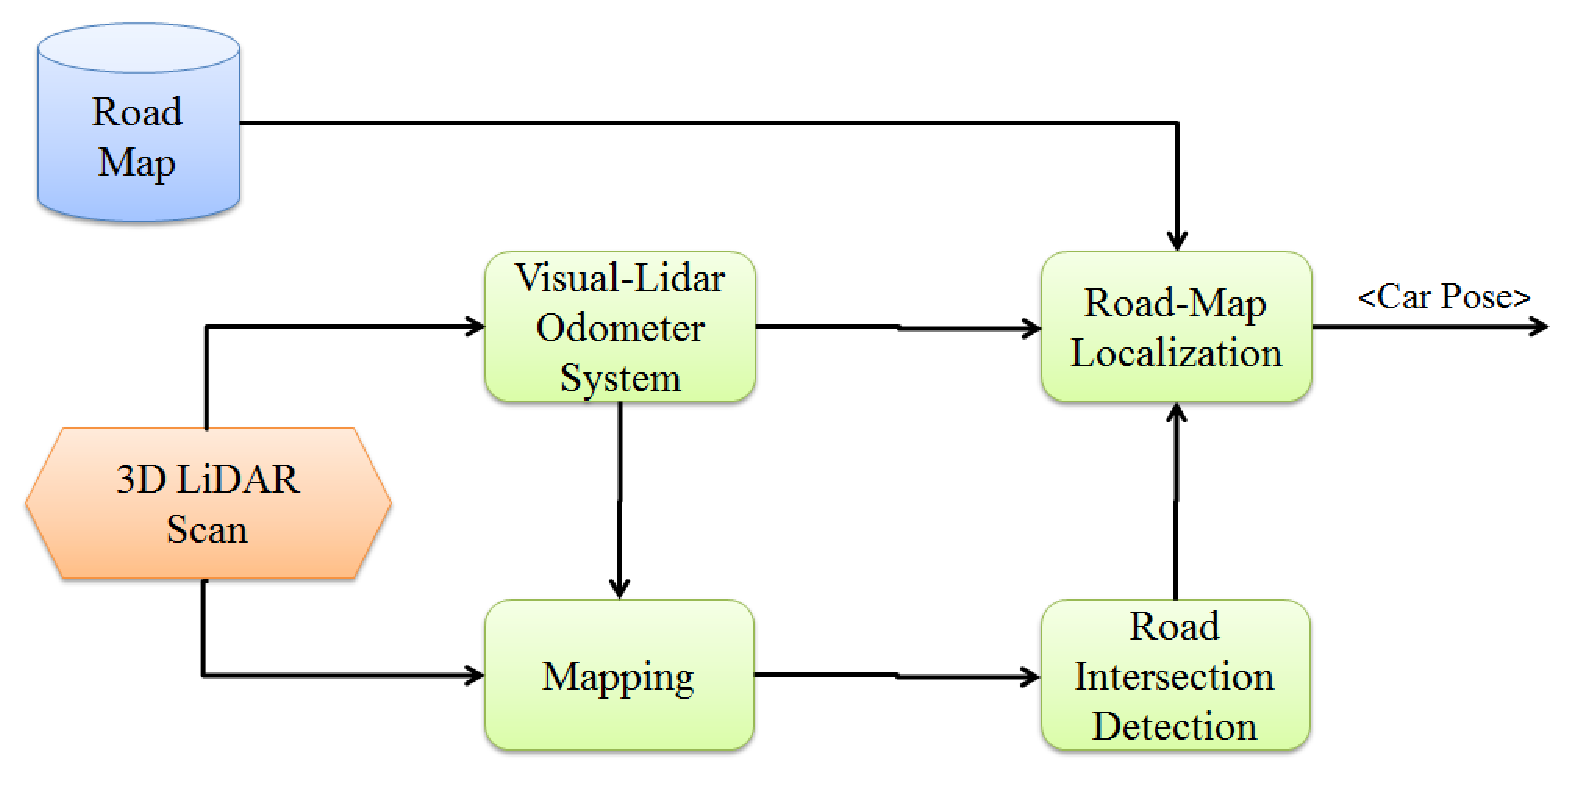
\includegraphics[width = 150mm]{RoadMap-system2.eps}
    \caption{Road-Map Localization System architecture. The system consists in road map and LiDAR sensing every instant that is used to estimate the car Odometries by Visual-LiDAR Odometer. Then, it uses this information to build re-emission and occupancy grid map locally as well as to build car path to compare against the road map. The maps are used by Road Intersection Detection sub-system to measure the road width, and inform whether car is crossing a road junction. The intersection observability is fused with distance between the dead-recking and road map by Monte Carlo Localization. Finally, the MCL computes the car pose selecting and summarizing the particles.}
    \label{Fig::RoadMap-system}
\end{figure}

To detect a road intersection formerly the 3D LiDAR data should be processed to produce local grid maps. The mapping builds a occupancy and re-emission grid map posing the lasers using dead-reckoning given by Visual-LiDAR Odometer. The Re-emission grid map is produced using the infrared LiDAR reflectance taking the average of re-emission value of each ray lied in a grid-cell. On the other hand, The occupancy map is made classifying whether a laser beam touch a obstacle or not. The both maps are used by the Road Intersection Detection sub-system to measure the road width and inform to MCL if the car is crossing a road junction. With this information, the MCL attributes a likelihood for each particle that is placed in intersection on the road-map. In the end, the particles are re-sampled by weight computed through intersection observability and comparison between the car path and road map. The selected ones are used to compose the car pose in the instant $t$.    


%Each particle poses the car path according to its position, and then it computes the weight. The road map could be downloaded from the Internet (Google or Bing maps), or produced by a segmentation on the area photographs.

\section{Bayesian Localization}

Bayesian methods \cite{Arulampalam02atutorial} allow adequate processing for dynamic state estimation problems. Bayesian approaches aim at synthesizing the probability density function (PDF) of the state vector based on all the available information. Consequently, vehicle global  localization can be treated as a Bayesian estimation problem, where the estimated variable is the pose of the vehicle. If the vehicle's pose (in the case of 2D localization) at time $k$ is expressed through the 3 DoF vector 

\begin{equation}
\label{Eq::ch2-1}
X_k = [x_k, y_k, \theta_k]
\end{equation}

then the localization problem implies the recursive synthesis of the PDF

\begin{equation}
\label{Eq::ch2-2}
p_{X_k, | z^{\left( k\right)}} = \left( X_k, | z^{\left( k\right)}\right) 
\end{equation}

where $z^{\left( k\right)}$ represents the sequence of all the available observations until time $k$.

If the posterior $p\left( X_{k-1} | z^{\left( k-1\right)}\right)$ $\left( *\right)$ at time $k-1$ is available, then the prior at time $k$ (due to a prediction step) is:

\begin{equation}
\label{Eq::ch2-3}
p\left( X_{k} | z^{\left( k-1\right)}\right) = \int  p\left( X_{k}, X_{k-1}\right) \cdotp p\left( X_{k} | z^{\left( k-1\right)}\right) \cdotp dX_{k-1}   
\end{equation}

where the conditional PDF $p\left( X_{k}, X_{k-1}\right)$ is provided by the process model of the system (in this case the kinematic model of the vehicle).

At time $k$ a set of measurements,  $z^{\left( k\right)}$, become available, consequently allowing the synthesis of a posterior that is obtained through a Bayesian update stage,

\begin{equation}
\label{Eq::ch2-4}
p\left( X_{k} | z^{\left( k\right)}\right) \propto p\left( X_{k} | z^{\left( k-1\right)}\right) \cdotp p\left( z^{\left( k\right)} | X_{k}\right)
\end{equation}

where $p\left( z^{\left( k\right)} | X_{k}\right)$ is the likelihood function associated to observation $z=z^{\left( k\right)}$.

For nonlinear non-Gaussian estimation problems, there are usually no analytic expressions for the estimated PDFs. A common approach for treating these problems is the Particle Filter (PF), that is able to estimate non-Gaussian and potentially multimodal PDFs. The generated PDF is represented through a set of samples (particles) with associated weights, and the estimates are computed based on these samples and weights. Details about PF can be found in \cite{Thrun:2005:PR:1121596, Thrun00j}

\section{Constrained Localization in Segment-Based Maps}

The system for localizing the platform is based on a process model and a set of likelihood functions that allow implementing the prediction and update steps of a PF. The process model is the kinematic model of the autonomous car employed in the experiments. And, in the context of this paper, there are two definitions of likelihood functions that are associated with the road segments: the Base Likelihood and the Extended Likelihood. The Base Likelihood is intended to model the likelihood of a position, i.e. the likelihood of a point being located on a valid road, while the Extended Likelihood (or path likelihood) is the likelihood of a path coinciding with a valid road. Both definitions of likelihood function are based on the segments defined in the road map.

\subsection{Base Likelihood Associated with the Road Map}

For a set of particles at time $k$, $\left\lbrace X_{k}^{i},w_{k}^{i} \right\rbrace _{i=1}^N$, the Base Likelihood (BL), $L_B\left(X_{k}^{i} \right)$, associated with a given map (set of segments) is defined as follows:
\begin{equation}
\label{Eq::ch2-5}
L_B\left(X\right) =p\left( map | X\right) = \max_{j=1}^{N}\left\lbrace f\left( X,S_j,C_j \right) \right\rbrace 
\end{equation}
where $\left\lbrace  S_j \right\rbrace_{j=1}^N$ represents the set of segments that compose the road map and $C_j$ denotes the properties of segment $S_j$ (road's width, number of lanes, lane directions, etc.). The function $f(\ldotp)$ is highly dependent on the distance between the pose component (of the state $X$) and the segment $S_j$. The function $f(\ldotp)$ may be also dependent on certain segment's properties such as its width and circulation direction.

A simplified version of \ref{Eq::ch2-5} is
\begin{equation}
	\label{Eq::ch2-6}
	L_B\left(X\right) =	p\left( map | X\right) = \left \{
		\begin{array}{l}
			1;\ if\ X\ \in\ \Omega(map,\Omega_k)\\\\
			0;\ if\ X\ \ni\ \Omega(map,\Omega_k)
\end{array}
\right.
\end{equation}
where the region $\Omega_k$ is a convex hull (usually just a rectangle) that contains the current set of particles at time $k$, i.e. $\left\lbrace  X_k^i \right\rbrace_{j=1}^N$.

The region $\Omega(map,\Omega_k)$ defines the roads as thick bands using the segment's locations and their associated properties provided in the road map definition. $L_B(X)$  is defined just on a small convex region of interest (ROI), $\Omega_k$, which is big enough to contain all the current particles. Through the dynamic definition of a moving and resizable ROI, the likelihood function $L_B(X)$ can be evaluated for all of the particles in real time at low computational cost.

\subsection{Extended Likelihood}

For improving the performance of the estimation process in the presence of out-of-map situations, an extended likelihood function is defined. An out-of-map situation occurs when the vehicle is traveling through unknown sections of the map, i.e. sections of the environment that are not included in the road map. 

Particles will tend to cluster towards regions of high Base Likelihood, which are assumed to be consistent with the map (e.g. existing roads in the map). This can be an adequate behavior in cases where the map is complete and the vehicle remains on it permanently. However, in certain cases, the vehicle might travel through roads that are not present in the road map. For those cases, the convergence of the localization process can be improved by using the recent history to build an estimated dead-reckoning path.

An estimated dead-reckoning path for each particle at time $k$ can be efficiently computed by combining dead-reckoning (obtained from an independent estimation process) with the current value of the particle $X_k^i$. This estimated path is only realistic for short time horizons, as dead-reckoning is accurate only for short time horizons. So, given a particle $X_k^i=[x_k^i,y_k^i,\theta_k^i]$ and recent dead-reckoning information, an estimated dead-reckoning path (it is actually a trajectory as well, since there is also time information), $\xi_i (t'), t' \in [k-\tau,k] $ is synthesized, where the value $\tau$ defines some short horizon of time. This path ends exactly at the current pose (i.e. matching position and heading) of the particle, i.e. $\xi_i(k)=X_k^i$.

The estimated dead-reckoning path is usually defined in a different coordinate system, as it is the result of an independent process (it could even be expressed in a completely uncorrelated coordinate frame). One important aspect of the estimated dead-reckoning path is its quality given a specific coordinate system, i.e. if its shape is, after proper rotation and translation, similar to the real path of the vehicle. If the estimated dead-reckoning path is expressed as the path $\mu^i (t' )=(x_{\mu}(t'),y_{\mu}(t'),\theta_{\mu}(t'))$, then the process of associating it with an individual particle and of mapping it into the global coordinate frame is performed simply by applying the rotation and translation defined by the current particle position and heading (see details in \cite{guivant2010robust}).

The Extended Likelihood (EL) of a particle is given by the line integral of the BL function along the estimated dead-reckoning path:
\begin{equation}
\label{Eq::ch2-7}
L_E (X_k^i )=\int_{k-\tau}^{k} L_B(\xi_i(t')) \cdotp dt',
\end{equation}
where $L_B (\xi)$ is the BL function of the point $\xi$, (as it was defined in \ref{Eq::ch2-6}).

In order to avoid the influence of the vehicle speed on the path likelihood, we evaluate BL according to the arc length parameter $s$, integrating over the path, (i.e., in space and not in time):
\begin{equation}
\label{Eq::ch2-8}
L_E (X_k^i )=\int_{0}^{l_s} L_B(\xi[s]) \cdotp ds,
\end{equation}
where $\xi[s]$ is the path expressed as a function of its intrinsic parameter $s$, and $l_s$ is the length of path. The continuous line integral of the path can be approximated by its discrete version,
\begin{equation}
\label{Eq::ch2-9}
L_E (X_k^i )=\sum_{j=1}^{N_J} L_B(\xi[s_j]) \cdotp ds,
\end{equation}
where the samples of the intrinsic parameter, $s_j$, are densely distributed over the estimated dead-reckoning path.

Some additional refinements can be considered for the definition of BL \ref{Eq::ch2-5}. For instance, one can consider the direction of the road. In this case, BL would not be just a function of the position, but it would depend on the vehicle heading at each point of the path. A path's segment that crosses a road would add to the likelihood if it crosses the road in the proper direction.

Figure \ref{Fig::ROI} shows a synthetic example of BL (shown in gray), particles that represent the pose of the vehicle, and their associated estimated dead-reckoning paths (in cyan). The particles' positions and headings are represented by blue arrows. The red path corresponds to the most likely hypothesis (according to the Extended Likelihood measure).

\begin{figure}[th]
\centering
    \subfloat[]{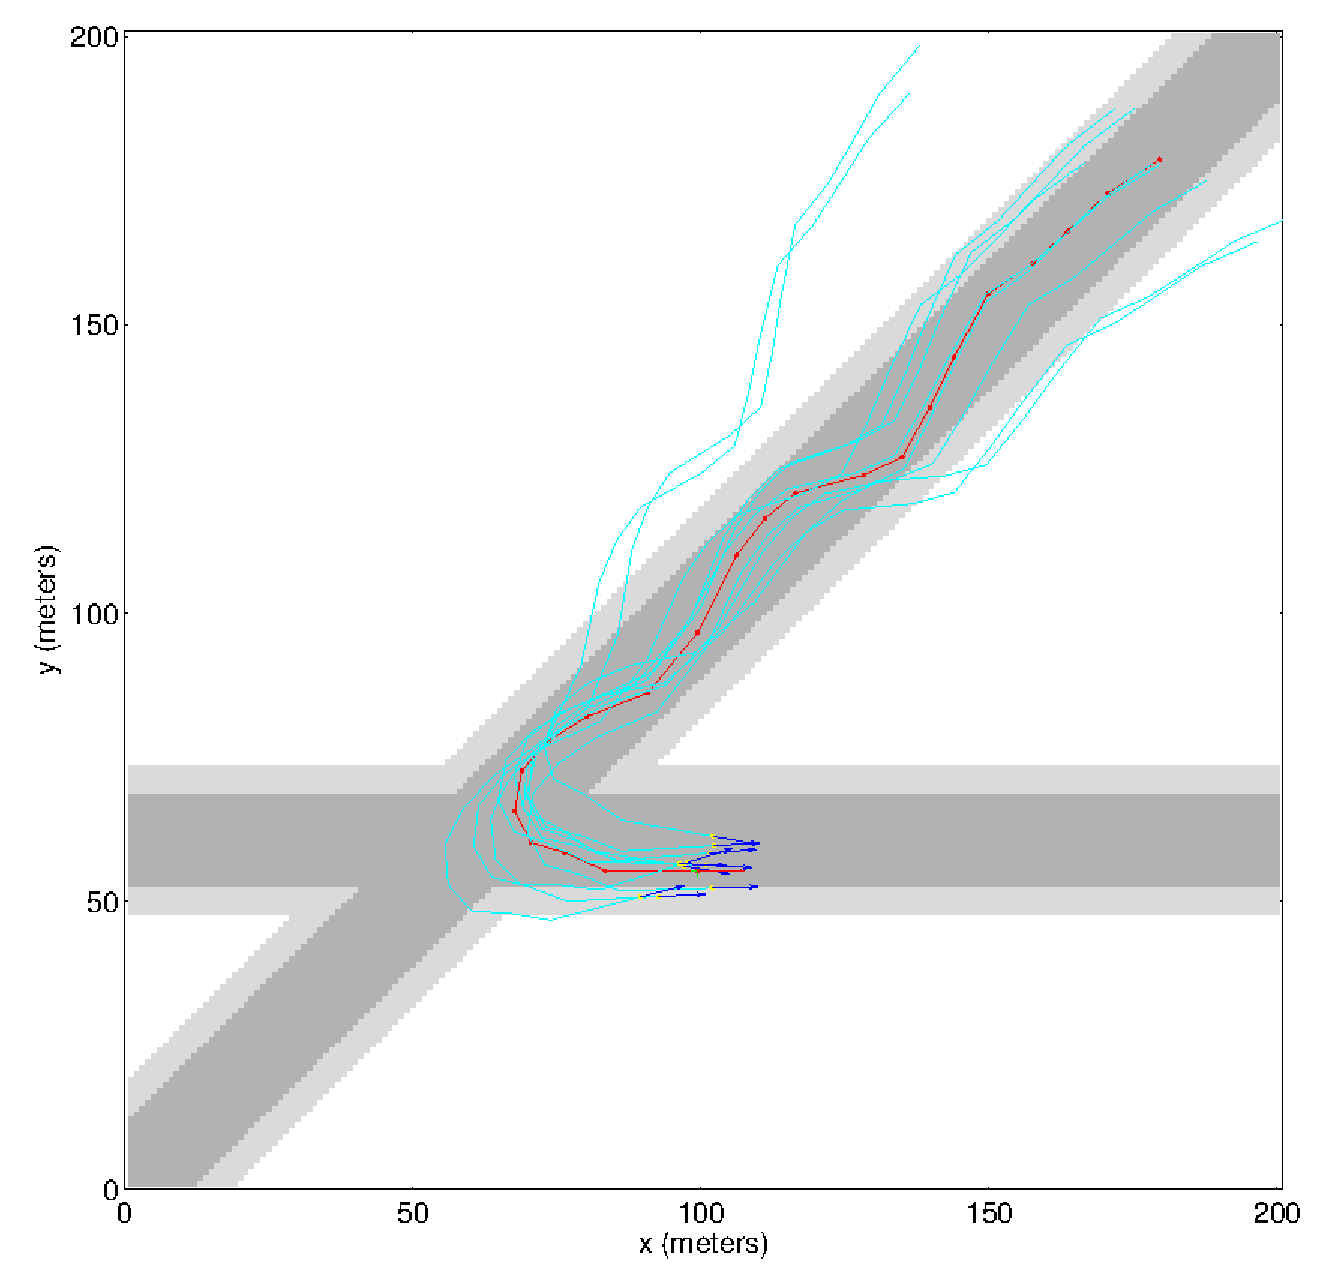
\includegraphics[width=50mm]{VGPSFig11.eps}
    \label{Fig::ROI1}}
    \subfloat[]{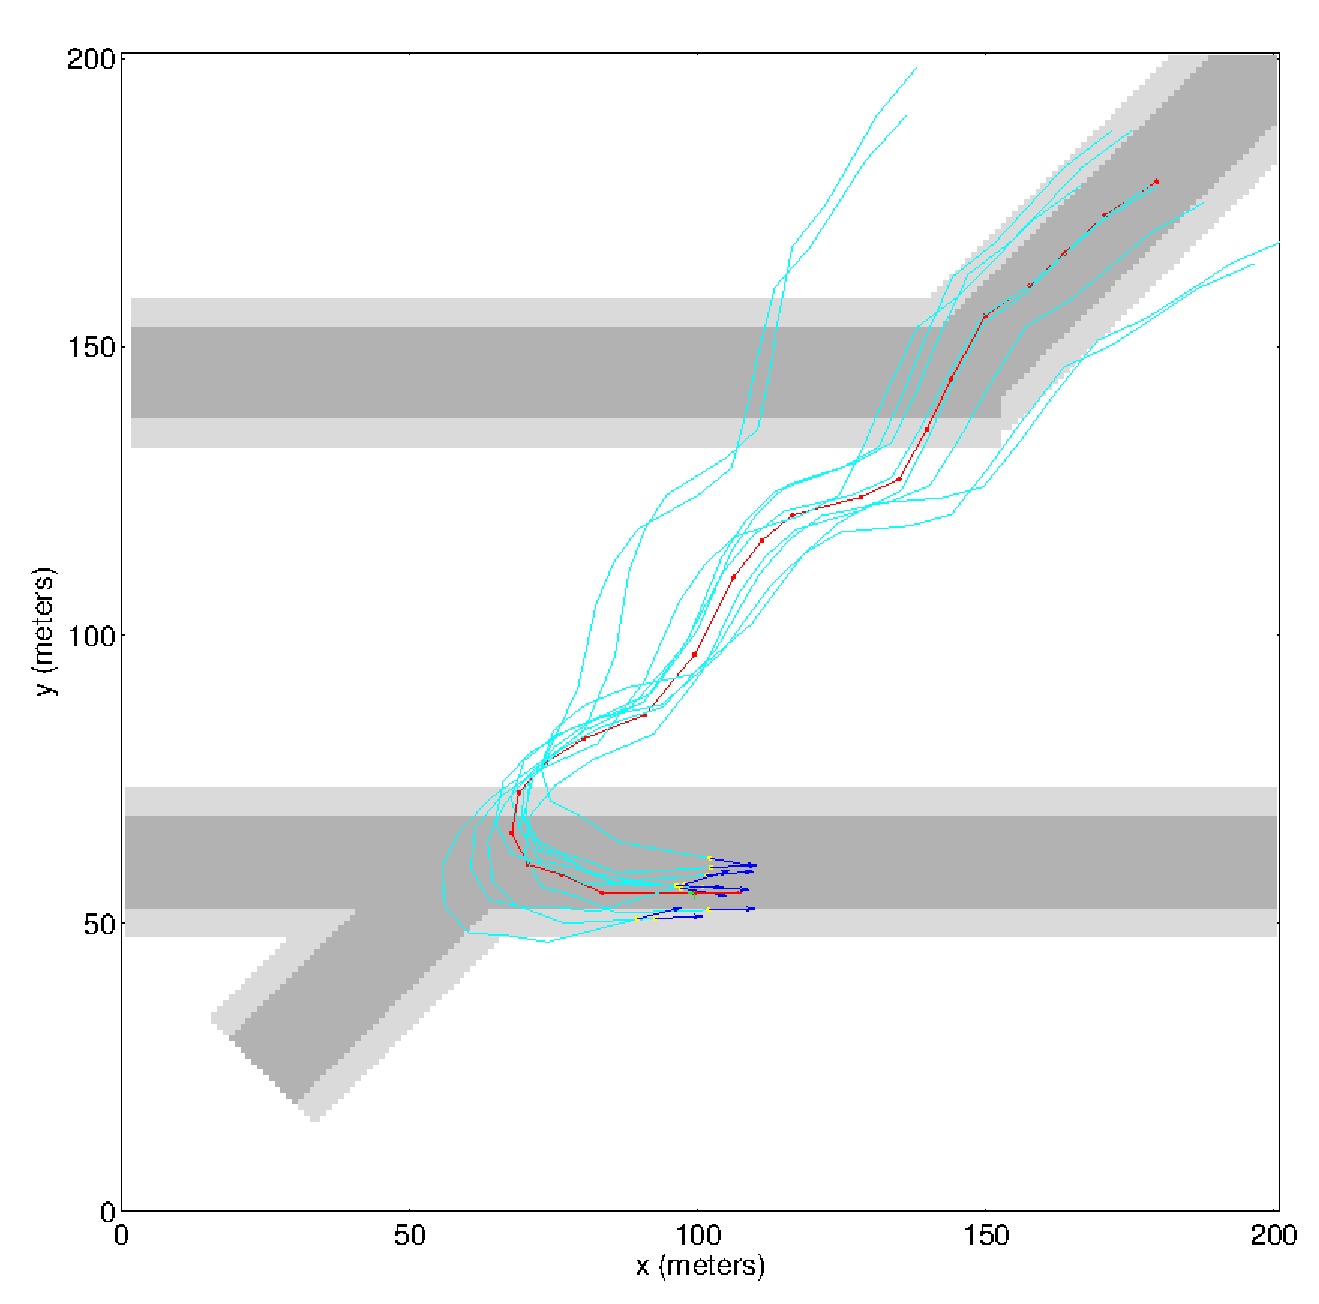
\includegraphics[width=50mm]{VGPSFig22.eps}
    \label{Fig::ROI2}}\\
    \subfloat[]{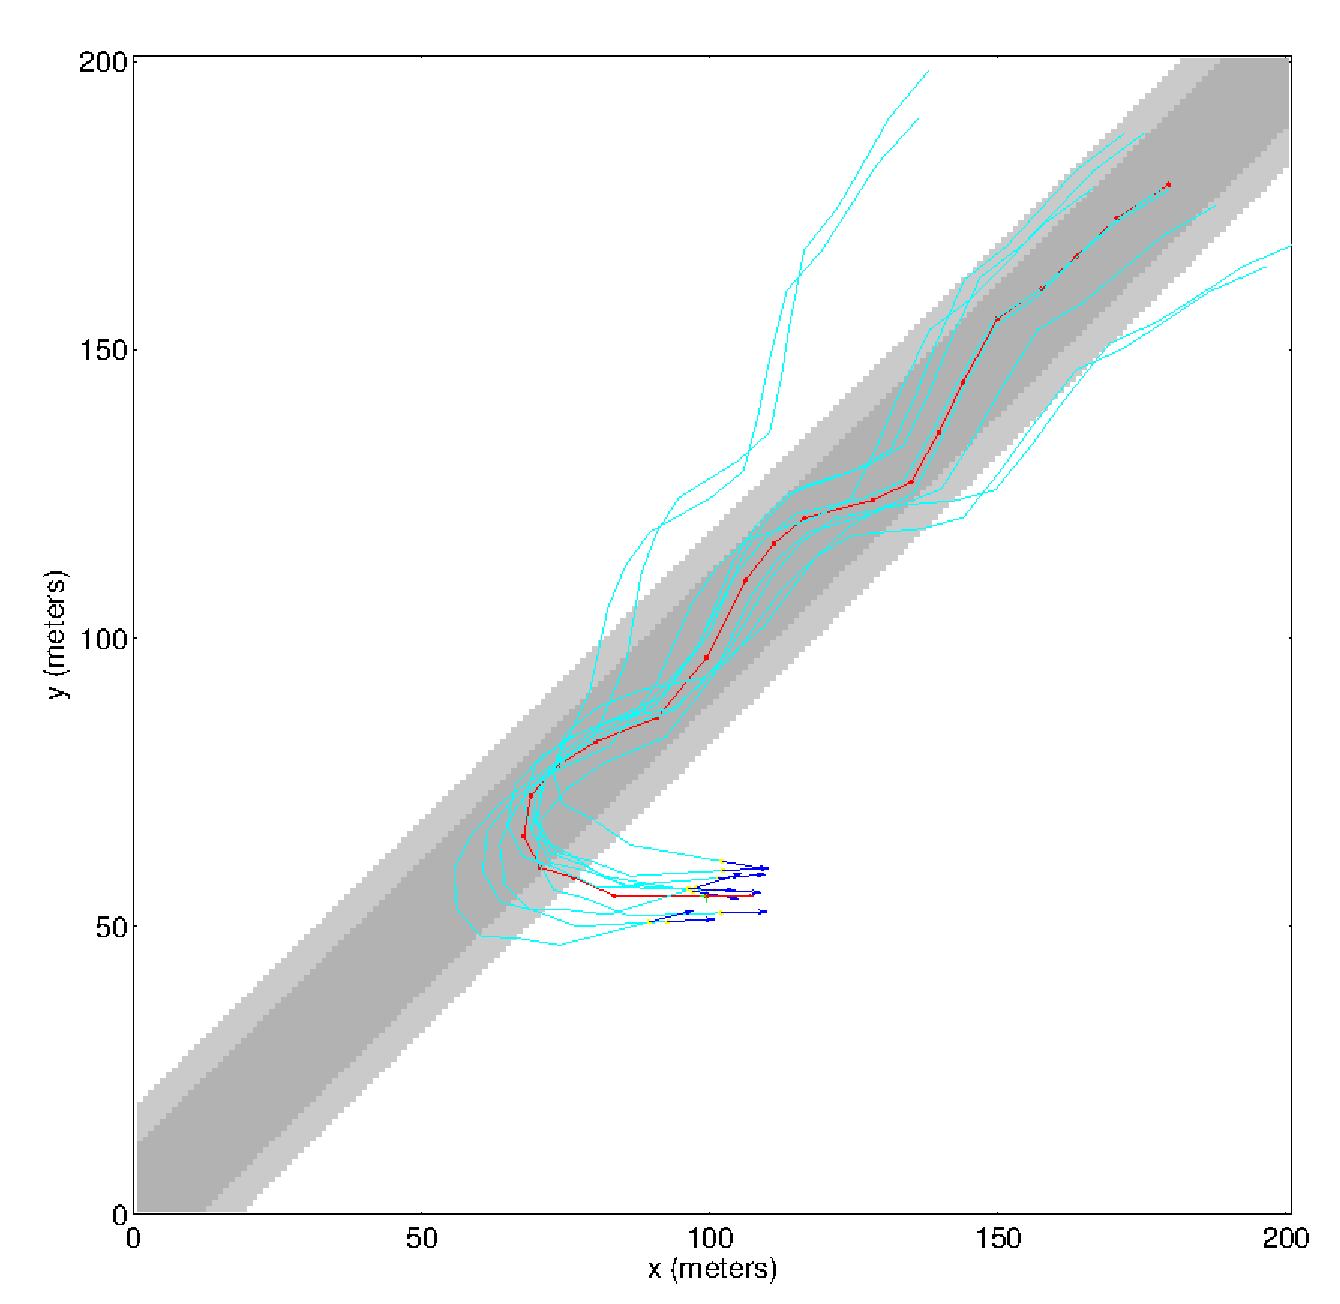
\includegraphics[width=50mm]{VGPSFig33.eps}
    \label{Fig::ROI3}}
    \subfloat[]{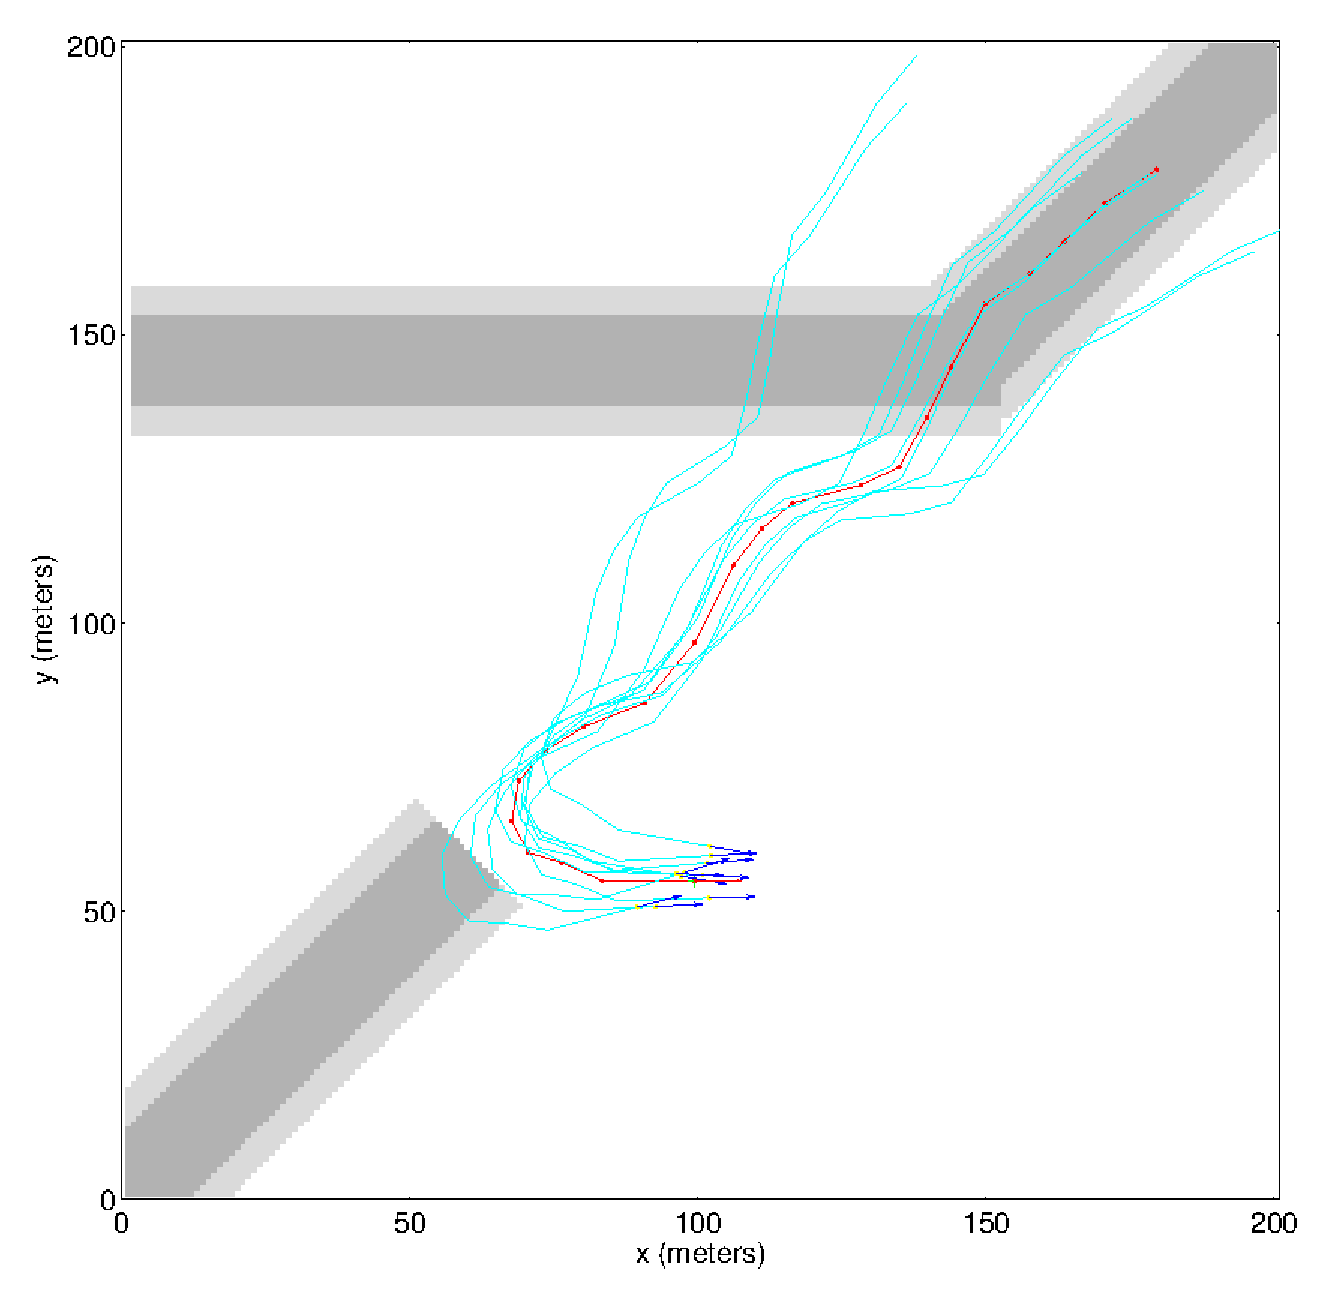
\includegraphics[width=50mm]{VGPSFig41.eps}
    \label{Fig::ROI4}}
\caption{Synthetic examples for a ROI of $200m\times200m$. The value of the Base Likelihood ($L_B(X)$) is shown in gray (the darker, the higher). A set of particles and their associated paths are included. The particle and path with maximum extended likelihood, $L_E(X_k^i)$ are shown in red. In three of the four cases, the vehicle temporarily abandons the road. In cases (b) and (c), all particles have equally low Base Likelihood; however, many particles still have high Extended Likelihood. Images taken from \cite{guivant2010robust}.}
\label{Fig::ROI} 
\end{figure}

By using observations that consider the estimated dead-reckoning path, the out-of-map problem is mitigated. The transition between a situation where the vehicle is on the road map to another where it is completely out of it (i.e. current pose and estimated dead-reckoning path are outside the road map) can be performed safely by using an approach based on hysteresis, as discussed in \cite{guivant2007global,guivant2010robust}.

In the synthetic example shown in Figure \ref{Fig::ROI}, the region of interest (ROI) is a square of 200 by 200 meters. This ROI is big enough to contain the current population of particles and their associated estimated dead-reckoning paths. The most likely particles are those that have a path mostly inside the road. In the case of Figure \ref{Fig::ROI4}, although all particles are located on the road (high Base Likelihood), many of their associated paths have large segments outside the zones of high Base Likelihood. In Figure \ref{Fig::ROI2} one can see the remarkable effect that a wrong heading direction may cause. This situation is also illustrated in \ref{Fig::ROI3}.

When the filter infers that the vehicle has been outside the map for sufficient time (i.e. no particle shows relevant part of their estimated dead-reckoning paths inside the road map), no updates are performed on the particles, i.e. the filter works in pure prediction mode. When the vehicle enters the road map again and there are enough particles with the required EL, i.e. higher than certain threshold, then the filter restart to apply updates on the particles. However, this transition typically is not immediate. There could be some delay until the required estimated dead-reckoning paths are consistent with the road map -- the fact that a particle is well inside a road of the road map does not mean that its likelihood should be high. It needs a relevant fraction of its associated estimated dead-reckoning path inside roads of the road map in order to be considered ``inside the road map''.


\subsection{Likelihood Based on Real Sensing Capabilities}

The previously defined likelihood functions are not based on real measurements (provided by sensors), i.e. the likelihood functions $L_B(x)$  and $L_E(x)$ are just based on the hypothesis that the vehicle is usually traveling on the roads of a known road map.

If the vehicle is equipped with proper sensors, it might be able to infer when it is effectively on a road or not (even though the road may not be part of the road map). This inference process could be based on 3D perception capabilities, such as the ones used in this work. Additionally, by processing the 3D sensor data, the vehicle may be able to infer if it is located nearby a road intersection or not. The detection of a road intersection is highly informative because it provides rich information for reducing the uncertainty of the estimates of the longitudinal position of the vehicle.

\subsection{Likelihood Associated with Road Intersections}

Different to the previously defined likelihood functions, the likelihood associated with the detection of road intersections is computed using observations of the real world. These observations just say that the vehicle is currently located in the vicinity of a road intersection, usually not specifying which one is it (e.g., no Data Association is available). However, this is not a problem because, although Data Association is desirable, it is not strictly necessary for identifying which intersection the vehicle is close to, since PF can deal with multi modal likelihoods.

The proposed likelihood function takes in consideration the probability false positives, i.e. the detection of road intersections that are not included in the road map. A simplistic 1D example of our likelihood function is shown in Figure \ref{Fig::Likelihood}. The fact that the value of the parameter B is higher than zero implies that this likelihood considers the possibility that a detected road intersection is not on the road map.

\begin{figure}[t!]
    \centering
    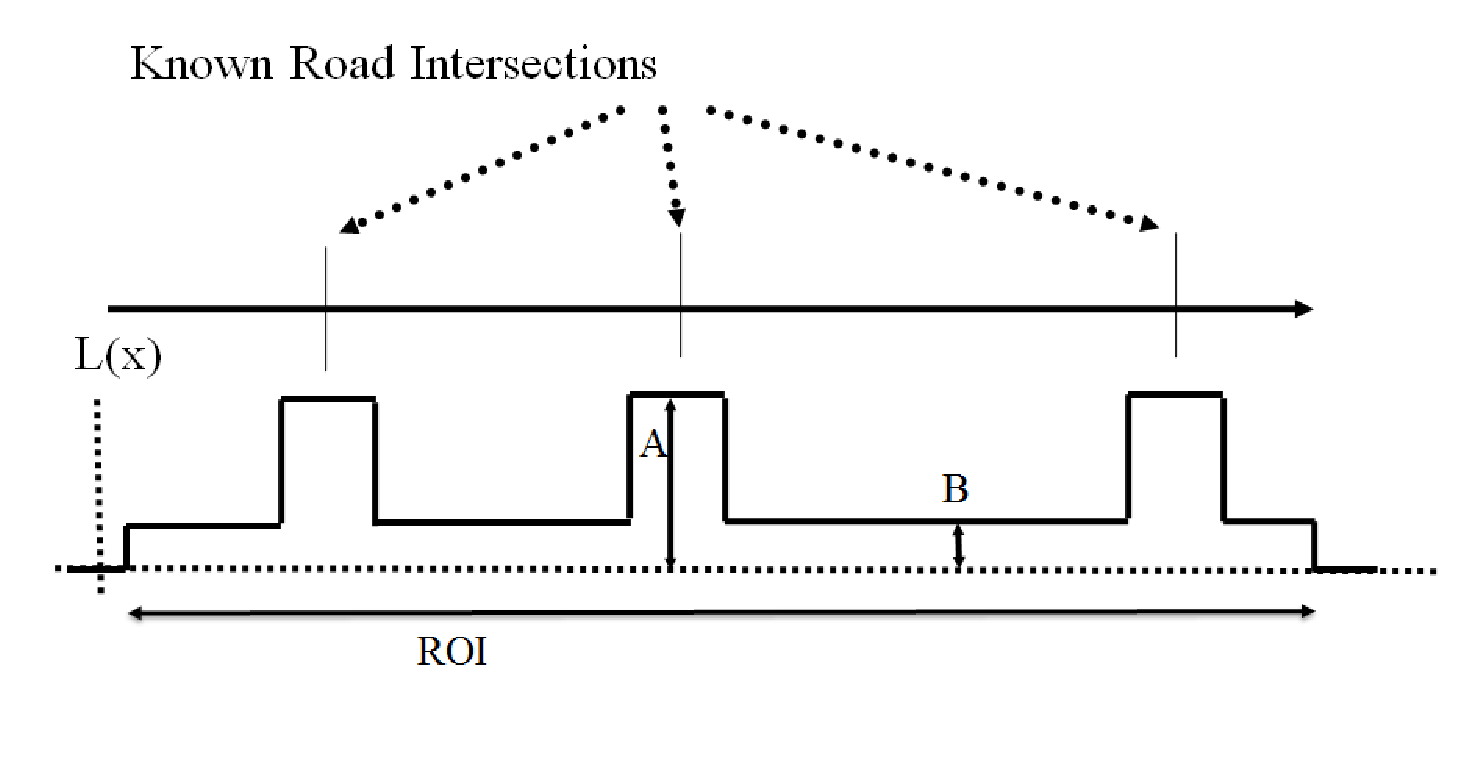
\includegraphics[width = 150mm]{Likelihood.eps}
    \caption{Likelihood $L(X)$ associated with the detection of a road intersection. $L(X)$ is equal to zero in any point outside the current ROI. Inside the ROI, it takes high values $(=A)$ at points that are close to known road intersections and low values $(= B,A\gg B>0)$ at points far from those known intersections.}
    \label{Fig::Likelihood}
\end{figure}

\section{Detection of Road Intersections Based on 3D Point Cloud}

Usually, there are diverse features that allow detecting a road intersection, such as traffic lights, pedestrian cross lanes, and also the pattern of the sites nearby. However, some of these characteristics may vary from cases of busy avenues to quiet neighborhood streets. Additionally, those are usually different in many countries as they have different rules and roads architecture. Therefore, techniques for inferring the proximity of road intersections should be based on some ``universally common'' feature, such as the boundaries of the roads themselves.

\subsection{Detection of Road Intersections}

The occupancy and re-emission grid map are used for detecting road intersections. But, a segmentation operation must be performed in the re-emission grid map (see Figure \ref{Fig::FIGURE_SEG_MAP1}) to highlight roads. For that, a simple threshold is used. To remove narrow regions of high re-emission (such as lane lines) the dilation morphological operation is employed. Figure \ref{Fig::FIGURE_SEG_MAP2} shows a typical result of our segmentation operation. This grip map is also used for the detection of road intersections and, from now on, we will call it simply filtered re-emission. 

\begin{figure}[t]
	\centering
	\subfloat[]{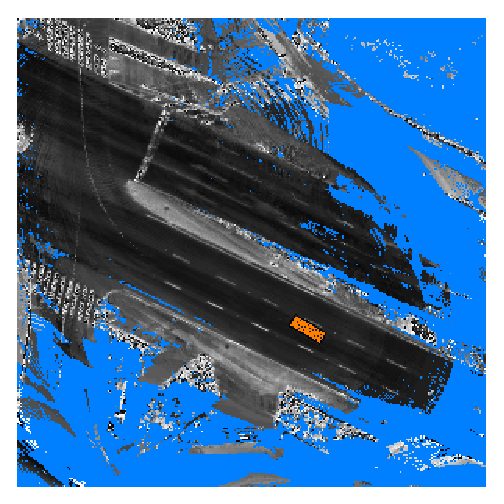
\includegraphics[width=42mm]{Remission1-1}
		\label{Fig::FIGURE_SEG_MAP1}}
	\subfloat[]{
\includegraphics[width=42mm]{segmented2-1}
		\label{Fig::FIGURE_SEG_MAP2}}
	\caption{Filtered Re-emission map. (a) Re-emission grid map built by averaging the infrared reflectance of laser targets associated with each cell. The blue cells in (a) represent the parts of the environment that have not been scanned by the sensor. (b) Road-map extracted from (a) by thresholding and dilation. The white areas are classified as road surfaces, while the blue areas are classified as non-road surfaces.}
	\label{Fig::FIGURE_SEG_MAP}
\end{figure}

The detection process is based on the road width that we estimate using these grid maps. Given the grid maps (that represent the current surroundings of the vehicle) and the estimated position and orientation of the vehicle on these grid maps, exploration lines are generated from the lateral boundaries of the vehicle in its transversal direction (i.e. perpendicular to the longitudinal direction of movements of the vehicle). Each exploration line is used to find the first obstacle in the set of map cells crossed by it. This allows the estimation of the distance between a point at the border of the vehicle and the first obstacle (see Figure \ref{Fig::FIGURE_ROAD_SIZE} for an illustration of the concept).

\begin{figure}[t]
	\centering
	\subfloat[]{
\includegraphics[width=42mm]{segmented1-2}
		\label{Fig::FIGURE_ROAD_SIZE1}}
	\subfloat[]{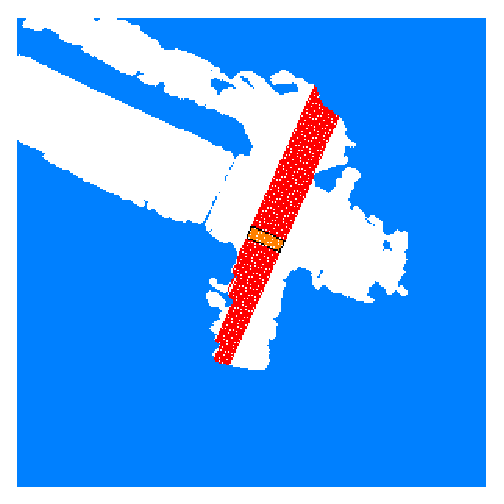
\includegraphics[width=42mm]{segmented1-1}
		\label{Fig::FIGURE_ROAD_SIZE2}}\\
	\subfloat[]{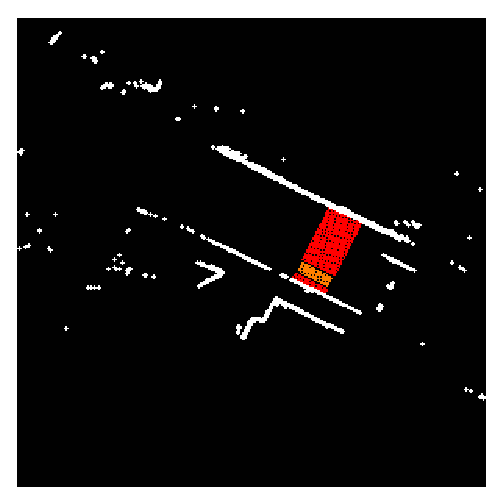
\includegraphics[width=42mm]{Occupancy2-1_black}
		\label{Fig::FIGURE_ROAD_SIZE3}}
	\subfloat[]{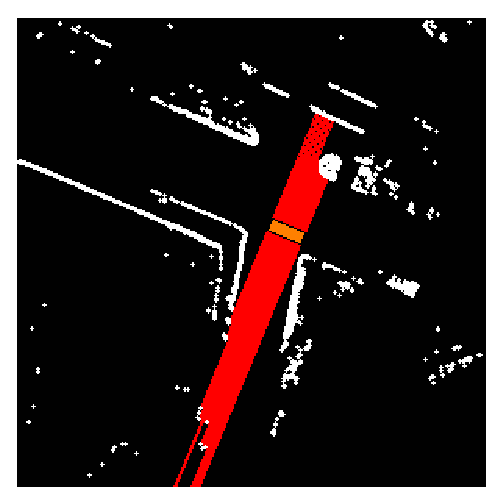
\includegraphics[width=42mm]{Occupancy2-2_black}
		\label{Fig::FIGURE_ROAD_SIZE4}}
	\caption{Transversal exploration lines. In red, the virtual scan performed by the transversal lines until they hit obstacles. The size of the lines is used to estimate the road width. The evolution of the estimated road width is used for inferring road intersections.}
	\label{Fig::FIGURE_ROAD_SIZE}
\end{figure}

This operation is performed on both sides of the vehicle. The pair of distances estimated for both sides allows estimating the width of the road. Each exploration line provides an instantaneous estimate of the road width, which is stored in a regressor. Exploration lines are not sampled by time but by space; consequently, the read width estimates are not affected by the speed of the vehicle.

Exploration lines are computed in both maps (occupancy grid map and filtered re-emission map), in order to mitigate the impact of the presence of other cars and imperfections in the filtered re-emission. The inferred width of the road is actually estimated as an average of the contents of the regressor (i.e., it is in fact a low pass filter). The use of these two maps is justified by the fact that they capture complementary information. In certain circumstances, the obstacle detection mechanism employed for building the occupancy grid  map cannot find any obstacle to infer the limits of the road, e.g. in cases of roads without curbs. However, in such cases, the re-emission information might still provide useful information to infer the boundaries of the road surface. In other situations, the re-emission information might be affected by traffic marks painted on the road surface, such as dense zebra crossing lines, but curbs might be present.

Even using both sources of information, there are cases when both are affected, e.g. when other cars (obstacles) are stopped nearby on the zebra lines during sufficient amount of time. Even in those cases, the inference process can avoid negative effects. Even though, in this context of application, the presence of false negatives (failure to infer a road intersection) is not crucial, while false positives (fictitious detection) would have a more negative impact. However false positives would still be tolerable by the localization process.

In order to reduce false negative during the intersection detection, the system does the correction by the intersection just when the particles are traveling close to one. To detect whether one particle is on a street junction or not, the same technique of exploration lines is applied for them in the road-map. As long as one particle is close to it, the system starts to evaluate the possibility of the car is on a road intersection. If the some particles have detected the intersection as well as the system, they will receive likelihood according to this, while the other ones the minimal likelihood. Consequently, during the particles resample the ones out of the intersection might be destroyed.






\chapter{Methodology and Experimental Setup}
\section{Introduction}

%A IARA é uma plataforma robótica experimental baseada em um automóvel de passeio adaptado. Esta adaptação envolveu a instalação no automóvel de: (i) mecanismos para controlar o acelerador, freio, posição do volante, etc.; (ii) sensores; (iii) computadores para receber os dados dos sensores e controlar o automóvel; e (iv) fontes de energia para os computadores e sensores.
%Após investigar inúmeras empresas no país e no exterior, a equipe do Laboratório de Computação de Alto Desempenho (LCAD) da UFES que desenvolveu a IARA não encontrou nenhuma empresa que oferecesse tecnologia similar ou superior à oferecida pela empresa norte americana Torc Robotics (http://www.torcrobotics.com) para o acionamento dos atuadores (volante, acelerador, freio, entre outros) do automóvel e disponibilização de energia elétrica para alimentação dos computadores e sensores necessários para os estudos pretendidos com a IARA (19). À época da aquisição, a tecnologia da Torc para veículos de passeio somente operava com o automóvel Ford Escape Hybrid. Assim, o LCAD importou este automóvel (Figura 8(a)) dos USA já com as tecnologias de acionamento e disponibilização de energia instaladas pela Torc (Figura 8(b)). 


\chapter{Experimental Results}

\section{Introduction}



\chapter{Conclusion e Future Works\label{cap:conclusao}}

% \vfill{}
% \begin{flushright}{}``\emph{Nada se cria, nada se perde, tudo se
% transforma.}''\\
% {\small Lavousier}\end{flushright}{\small \par}
% \vfill{}

% Neste cap�tulo � apresentado as conclus�es e alguns trabalhos futuros
% ...
\newpage


\section{Conclusion}

{\bf Alguns itens interessantes para a conclus�o de um projeto de gradua��o}


\section{Future Works}

\appendix


%\chapter{Ground-Truth Generation Based on Graph-SLAM}
\label{sec:Mapping}

This system was design aims to generate a ground-truth of large-scale urban environment. The system has been used also to achieve a high quality pose estimation to address the problem to map large-scale urban environment. It was developed during the development of this thesis and has been apply in our in house autonomous car to create maps that will be used to localize the car during autonomously navigation. It was named as Large-Scale Environment Mapping System (LEMS).
  
The architecture of the Large-Scale Environment Mapping System (LEMS) is illustrated in Figure \ref{Fig::FIGURE02}. In the first step, GPS and odometry are used as input to an odometry calibration subsystem. This subsystem calculates the odometry biases and outputs the corrected odometry. After that, the data from all sensors, the calibrated odometry, GPS, IMU and Velodyne readings are synchronized by the time of the slowest sensor (in this case, the Velodyne). At this stage, for each Velodyne reading, there are associated data from the other sensors. It is fundamental to guarantee that the Velodyne reading and the data used to calculate its poses are  consistent in time.

\begin{figure}[ht]
    \centering
    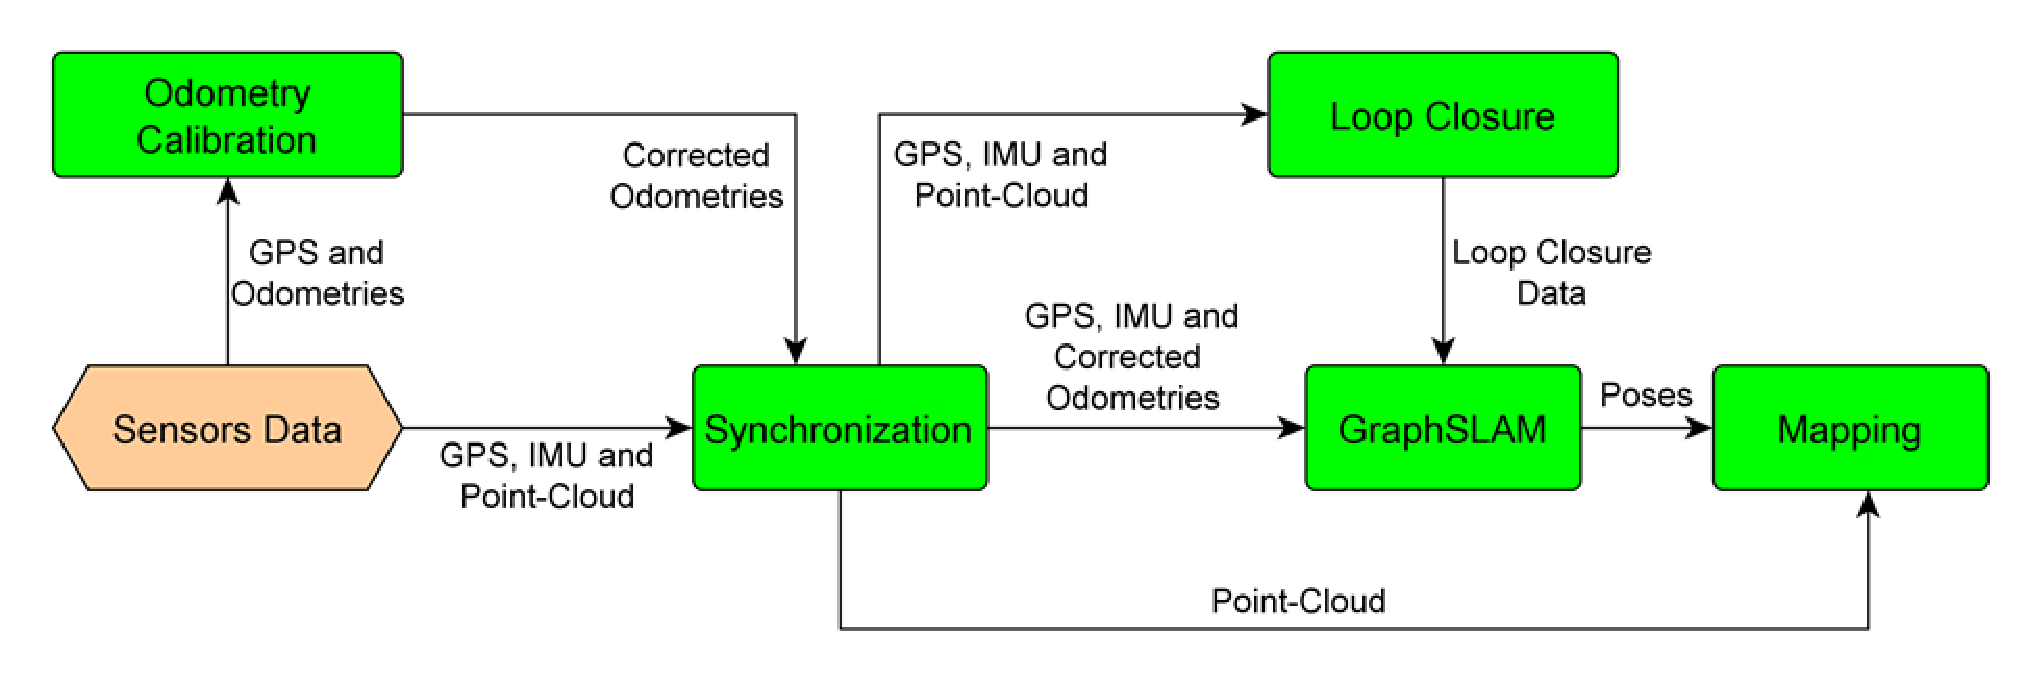
\includegraphics[width = 120 mm]{FIGURE02}
    \caption{Large-Scale Environment Mapping System (LEMS) Architecture. Firstly, a human drives IARA through the interest region and the sensor data are logged. Then, the Odometry Calibration subsystem is executed to remove systematics errors in the odometry data. After that, the data from all sensors are synchronized by the Velodyne time-stamp (slowest sensor) and the Loop Closure subsystem is used to detect revisited regions and to measure the displacement between the poses in the subsequent visits. Finally, the GraphSLAM subsystem is executed to estimate a feasible vehicle path and the Mapping subsystem is executed to build the environment grid map by projecting the velodyne point cloud from 3D to 2D, detecting obstacles, and placing them in the world using the GraphSLAM poses.}
    \label{Fig::FIGURE02}
\end{figure}

The Loop Closure subsystem receives as input the data from GPS, IMU and  Velodyne, detects loop closure regions and estimates the displacement between the poses in the subsequent visits to the same region. The output of the loop closure subsystem, the data from GPS, IMU and the calibrated odometry are used to introduce restrictions to the GraphSLAM optimizer that is responsible for calculating the set of most likely poses given sensor data. Lastly, the mapping subsystem receives as input the Velodyne point clouds and the respective poses, calculated by the GraphSLAM, and outputs the environment occupancy grid map. It is important to note, however, that the proposed architecture can be easily extended to create any kind of grid map (e.g., remission grid maps, likelihood field grid maps, etc.).

\subsection{Pre-Processing}

The vehicle's odometry data is composed of the velocity ($V_t$) and the steering wheel angle $\Phi_t$ for each instant $t$. The data is subject to three biases: a multiplicative bias in the wheel velocity measurement ($B_V^*$), a multiplicative bias and a additive biases in the steering wheel angle ($B_\Phi^*$ and $B_\Phi^+$, respectively). The velocity component has no additive bias due to the precise zero measurement in vehicle odometry. The incorporation of an additive velocity bias would lead to false movement measurements when the vehicle is stopped. Given these definitions, the corrected wheel velocity $V_t'$ and the corrected steering wheel angle $\Phi_t'$ are:

% % % % % % % % % % % % % % % % % % % % % % % % % % % % % % % % % %
% @Filipe: checar como tirar o espaco branco em cima da equacao.
% % % % % % % % % % % % % % % % % % % % % % % % % % % % % % % % % %

\begin{equation}
\label{Eq::velocity}
V_t' = V_t B_V^*
\end{equation}
\begin{equation}
\label{Eq::phi}
\Phi_t' = \Phi_t B_\Phi^* + B_\Phi^+
\end{equation}

To calculate the biases, we used an evolutionary optimization algorithm. The objective function was defined as the Mean of Squared Errors (MSE) between the dead-reckoning poses (calculated using the intermediary value of the biases) and the GPS poses:

\begin{equation}
\label{Eq::MSE}
e = \frac{1}{N}\sum_{t}\left( Y_t-G(V_t', \Phi_t')\right) ^2
\end{equation}

where $G(.)$ is the vehicle's motion model that outputs the dead-reckoning at instant $t$, $Y_t$ is the GPS measurement at the instant $t$, and $N$ is the number of poses. This objective function reflects the fact that in an error-free situation, each dead-reckoning pose should be inside the circle centered in the respective GPS measurement and with radius given by the GPS standard deviation.

Since GPS data has a lack of orientation, the initial angle of the robot was added as an additional variable to the optimization problem. During the experiments it was observed that optimizing the initial angle provides better results than using the angle provided by the IMU due to its high angular error.

To perform the optimization, it was used the evolutionary algorithm known as Global Best Particle Swarm Optimization (GBEST-PSO) \cite{53eberhart1995new, 70clerc2002particle, 71de2009swarm}. In our application, each particle represents a set of biases ($B_V^*$, $B_\Phi^*$ and $B_\Phi^+$) and the initial angle of the vehicle. The optimization starts by setting random possible biases and angle values to the particles. Then, the objective function (also known as fitness function in evolutionary algorithms) is calculated for all the particles. It consists of integrating the biases to the odometry data, calculating the dead-reckoning, and comparing the dead-reckoning with the GPS poses using Equation \ref{Eq::MSE}. The particle with the dead-reckoning that best fits the GPS path becomes the global best (GBEST), and all other particles move in direction to the best values found so far. After the movements, some other particles can find better values and become the new GBEST. These steps are repeated until a pre-defined maximum number of iterations is reached.

In the GBEST-PSO, each particle moves from its best individual position (Particle Best – PBEST) to the global best position (GBEST). The GBEST is defined as the highest fitness position found during all the optimization iterations. To perform the movements, the particles are submitted to a random acceleration with direction given by the vector connecting the PBEST and GBEST positions. This acceleration changes the particle velocity, and the new velocity is used to update the particle position. The PSO velocity and position updating rules are \cite{70clerc2002particle}:
\begin{equation}
\label{Eq::PSOVelocity}
W_i(k+1)=\lambda \left[ W_i(k)+C_1 R_1 \left( P_{Best_i} - I_i(k)\right) +C_2 R_2 \left( G_{Best}-I_i(k)\right) \right]
\end{equation}
\begin{equation}
\label{Eq::VelocityUpdate}
I_i(k+1)=I_i(k)+W_i(k+1)
\end{equation}
where $\lambda=\frac{2}{2-\varphi-\sqrt{\varphi^2-4\varphi}}$ with  $\varphi = C_1+C_2$, $\varphi>4$.

Here, $I_i = [I_{i1}, I_{i2}, ..., I_{in}]^T$ is the position of the $i^{th}$ particle in a n-dimensional  search space (in this work, $n=4$) and $W_i = [W_{i1}, W_{i2}, ..., W_{in}]^T$ is the velocity of the $i^{th}$ particle. $P_{Best_i}$ is the position with maximal fitness visited by the $i^{th}$ particle and $G_{Best}$ is the position with maximal fitness found by all particles during all iterations. $\lambda$ is a constriction factor, and $C_1$ and $C_2$ are positive constants. $R_1$ and $R_2$ are random values in the range $[0,1]$ generated by uniform probability distribution. In \cite{70clerc2002particle}, the authors analyze what are the best values for these parameters and they found that $\varphi$ equals to $4.1$, $\lambda=0.729$, and $C_1=C_2=2.05$ are appropriate ones. In this work, we used these values for the parameters.

\subsection{Loop Closure}

The loop closure subsystem has two objectives: firstly, to detect the poses of the robot when it revisits a region, and secondly, to measure the displacement of the poses in relation to the first visit caused by the dead-reckoning accumulated error.

To detect whether some region has already been visited, each GPS position data is compared with older GPS positions. If some old position has a smaller distance from the current GPS position than a pre-defined threshold (five meters, in this work) and the timestamp difference is bigger than a pre-defined threshold (in this work two minutes is used), a new loop closure is detected. In this case, both positions (the current one and the old one) are sent to the displacement measurement phase. If more than one position satisfies the loop closure condition, only the closest one is considered. We use GPS to detect loop closure poses because the GPS uncertainty is constant over time and does not grow even if the robot travels long distances.

To estimate the displacement between two loop closure poses, we translate the Velodyne point clouds to the poses given by the GPS positions and the IMU orientations. Then, we register the point cloud of the second visit to the point cloud of the first visit using the GICP. This algorithm estimates the correction transformation that best fit a source point cloud to a target point cloud.

\subsection{GraphSLAM}

The GraphSLAM is a full-SLAM algorithm \cite{10thrun2006graph} in which the probabilistic variables are represented by graph vertices, and the sensor measurements are represented by graph edges. In this work, each vertex represents a robot pose (x-y and $\theta$) and edges correspond to sensor measurements and its uncertainties (represented as covariance matrices). Note that the GraphSLAM edges are the dead-reckoning, the loop closures and the fused data from the GPS and IMU (GPS/IMU). Figure \ref{Fig::FIGURE03} illustrates an example of a graph.

\begin{figure}[ht]
    \centering
    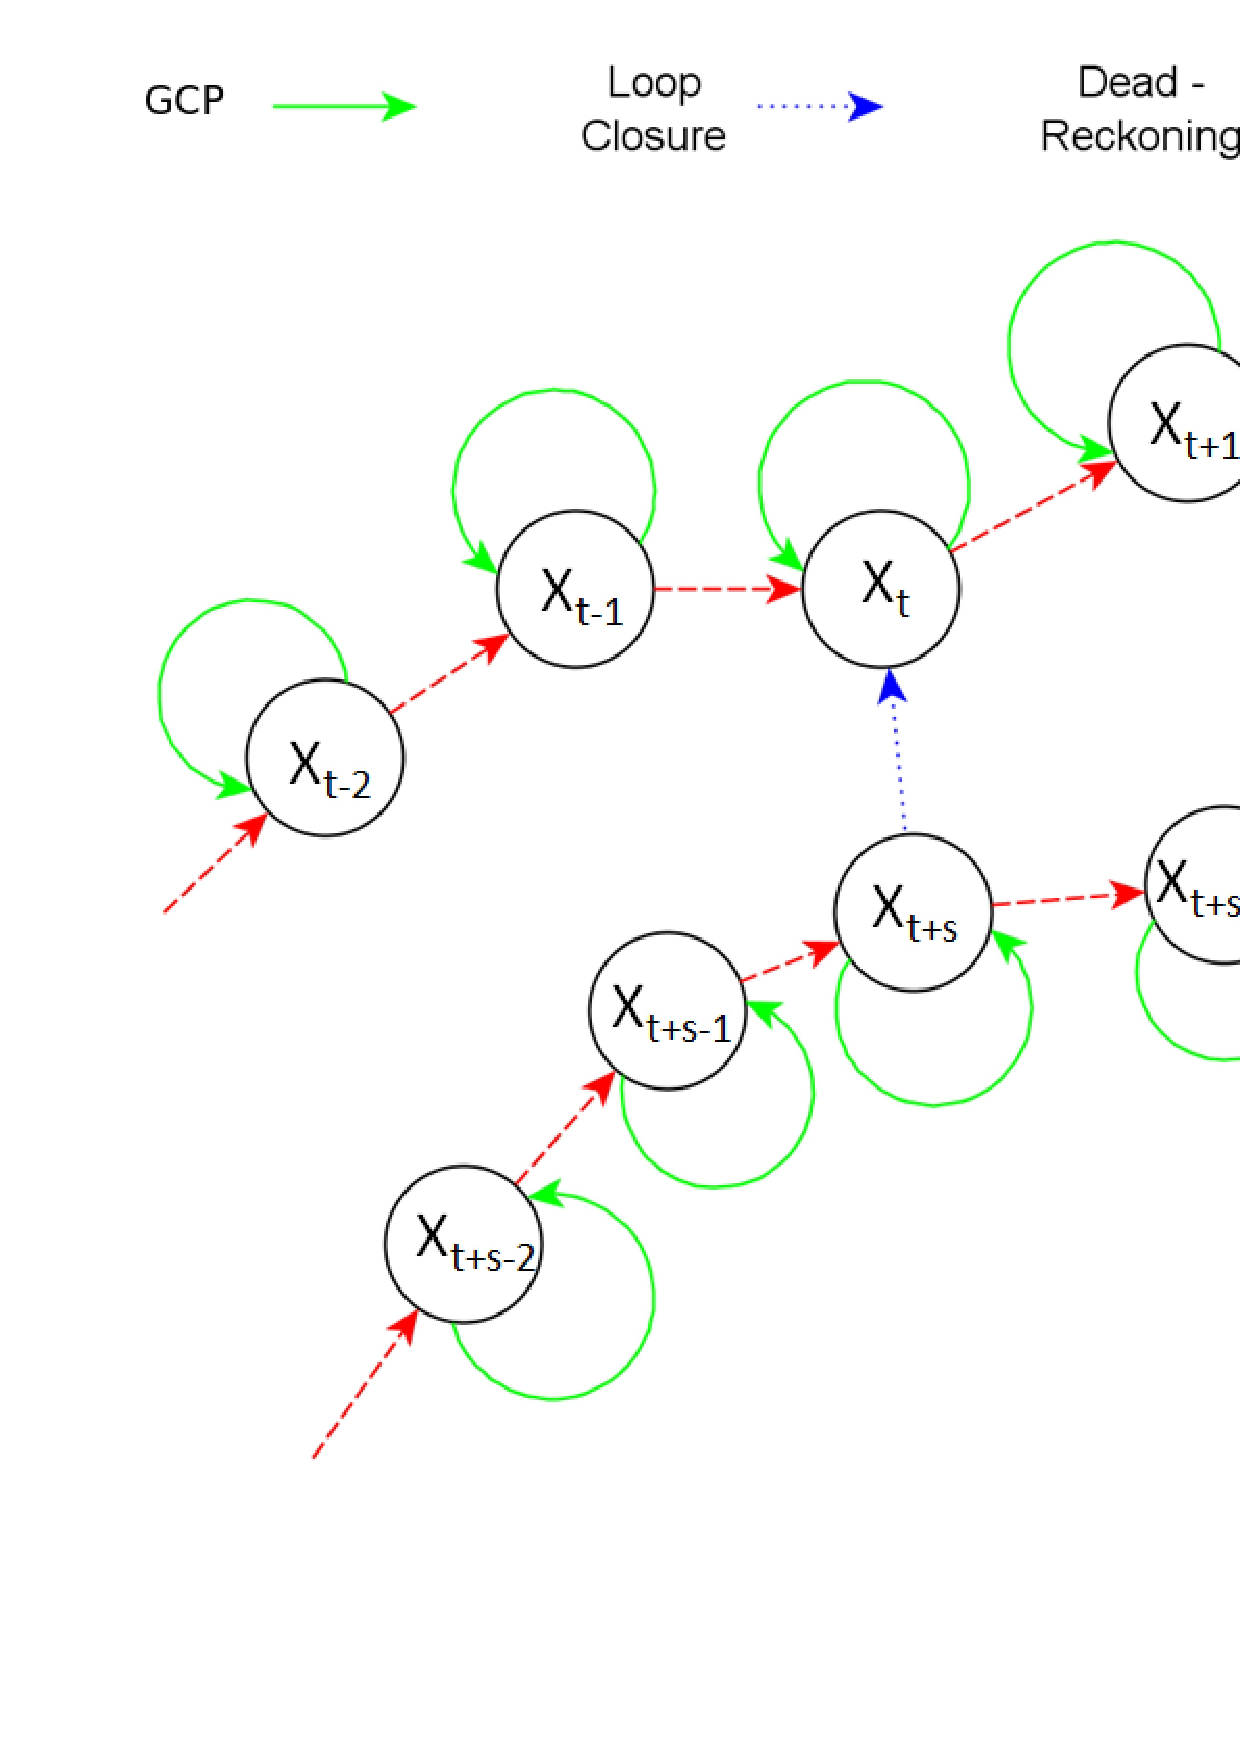
\includegraphics[width = 100 mm]{FIGURE03}
    \caption{Example of Graph Constructed by GraphSLAM. The black circles represent the poses, the red dashed edges represent the dead-reckoning displacements between two consecutive poses, the green filled unitary edges represent the GPS/IMU measurements, and the blue dotted edges represent the loop closures restrictions.}
    \label{Fig::FIGURE03}
\end{figure}

To estimate the most likely poses given the graph, several maximum-likelihood estimation techniques can be used. In special, when the sensor uncertainties are Gaussian, the maximum-likelihood estimation problem can be translated in a quadratic optimization problem solvable by gradient-based algorithms. The objective function of our GraphSLAM version is given by:
\begin{equation}
\label{Eq::GSLAMOBJ}
J=R_O+R_G+R_L
\end{equation}
where $R_O$ is the sum of odometry restrictions, $R_G$ is the sum of GPS/IMU restrictions, and $R_L$ is the sum of loop closure restrictions.

Because dead-reckoning and loop closure leads to Gaussian displacement restrictions and GPS/IMU lead to Gaussian global position restrictions, the log-likelihood objective function can be defined as:
\begin{equation}
\label{Eq::GSLAMlikelihoodOBJ}
\begin{array}{c}
J = \sum_{t}\left[ (X_t-(X_{t-1}+\delta_{t-1, t}))^TQ_t^{-1}(X_t-(X_{t-1}+\delta_{t-1, t}))\right]  \\
 + \sum_{t}\left[ (X_t-Y_t)^T R_t^{-1}(X_t-Y_t)\right]  \\
 + \sum_{X_A,X_B\in Loops}\left[ (X_B-(X_A+\delta_{X_A, X_B}))^TS_{X_A,X_B}^{-1}(X_B-(X_A+\delta_{X_A, X_B}))\right]
\end{array}
\end{equation}
where $X_t$ is a pose in time $t$,  $\delta_{t-1, t}$ is the estimated displacement between two consecutive poses $X_{t-1}$ and $X_t$ from dead-reckoning, $Y_t$ is a GPS/IMU measurement in time $t$, $\delta_{X_A, X_B}$ is a displacement from the pose $X_A$ to the pose $X_B$ (estimated by GICP) and $Q_t^{-1}$, $R_t^{-1}$ e $S_{X_A,X_B}^{-1}$ are the inverse covariance matrices from dead-reckoning, GPS/IMU and loop closure, respectively. During the optimization, the poses ($X_t$,$X_{t-1}$, $X_A$ and $X_B$) are changed and the sensors observations ($\delta_{t-1, t}$, $Y_t$ and $\delta_{X_A, X_B}$) and covariance matrices ($Q_t$, $R_t$ and $S_{X_A,X_B}$) stay fixed.

It is important to point out some technical details about our framework. Firstly, to calculate the vehicle motion (x-y and $\theta$) from the odometry data (velocity and steering angle) we used the Ackermann motion model \cite{50wickens2005fundamentals}. Secondly, once GPS/IMU data present bounded uncertainties, they were used to initialize the robot poses and to restrict the optimization search space.



% @Filipe: This command is used to lock the figures in the section they were declared.
%\FloatBarrier



\bibliographystyle{abnt-alf}
\bibliography{dissertacao}




\end{document}

\end{document}
